\documentclass{llncs}
\usepackage[latin1]{inputenc}
\usepackage{amsmath}
\usepackage{amsfonts}
\usepackage{amssymb}
\usepackage{algorithm}
\usepackage{algorithmic}
\usepackage{url}
\usepackage{xcolor,colortbl}
%\usepackage{geometry}
\usepackage{subfigure}
\usepackage[font=small,labelfont=bf]{caption}

% Normal
%\geometry{hmargin = 4cm, vmargin=3.8cm}
% New for submission
%\geometry{hmargin = 3.2cm, vmargin=2.9cm}




%\definecolor{Gray}{gray}{0.85}



%%%%%%%%%%%%%%%%%%%%%%%%%%%%%%%%%%%%%%
%\theoremstyle{definition}
%\newtheorem{teo}{Theorem}[section]
%\newtheorem{defi}{Definition}[section]
%\newtheorem{oss}{Remark}[section]
%\newtheorem{lemma}{Lemma}[section]
%\newtheorem{cor}{Corollary}[section]
%\newtheorem{ex}{Example}[section]
%\newtheorem{prop}{Proposition}[section]
%\newtheorem{note}{Notes}[section]
%\newtheorem{fact}{Fact}[section]

\spnewtheorem{assumption}{Assumption}{\bfseries}{\itshape}
\spnewtheorem{notation}{Notation}{\bfseries}{\itshape}





%
\newcommand{\sensVar}{z}
\newcommand{\sensRandVar}{Z}
\newcommand{\sensVarSet}{\mathcal{Z}}
\newcommand{\plaintext}{p}
\newcommand{\randPlaintext}{P}
\newcommand{\plaintextSet}{\mathcal{P}}
\newcommand{\targetFunction}{e}


\newcommand{\key}{k}
\newcommand{\randKey}{K}
\newcommand{\keyTest}{k^{\star}}
\newcommand{\keySet}{\mathcal{K}}
\newcommand{\var}[1]{\mathrm{Var}\left(#1\right)}

\newcommand{\numTraces}[1][z]{N_{#1}}
\newcommand{\numTracesAttack}{N_a}
\newcommand{\sss}[2][z]{\textbf{x}^{#1}_{#2}} % $\sss{i}$ or $\sss[k]{i}$
\newcommand{\sssTest}[2][z]{\textbf{y}^{#1}_{#2}} % $\sssTest{i}$ or $\sssTest[k]{i}$
\newcommand{\SSS}[1][z]{\textbf{X}^{#1}}
\newcommand{\sssSet}{\mathcal{X}}
\newcommand{\SSSTest}[1][z]{\textbf{Y}_{#1}}

\newcommand{\extractor}[2][]{\varepsilon_{#1}(#2)}
\newcommand{\extract}{\varepsilon}
\newcommand{\bestExtractor}{\varepsilon^\star}

\newcommand{\AAlpha}{\boldsymbol\alpha}
\newcommand{\BBeta}{\boldsymbol\beta}
\newcommand{\mmm}{\textbf{m}}
\newcommand{\mmmX}{\overline{\textbf{x}}}
\newcommand{\mmmXclass}[1][z]{\overline{\textbf{x}}^{#1}}
\newcommand{\mmmY}{\overline{\textbf{y}}}
%\newcommand{\mmmX}[1][z]{{\bf \meanEst{{\textnormal{$(#1)$}}}}}
%\newcommand{\mmmY}[1][z]{{\bf \meanEst{{\textnormal{$(#1)$}}}}}

\newcommand{\mmmXtot}{{\overline{\bf \meanEst{}}}}

\newcommand{\meanNoise}{{\bf \mu}}
\newcommand{\meanEst}[1]{\mathrm{\bf m}_1 #1 }
\newcommand{\varEst}[1]{\mathrm{m}_2(#1)}
\newcommand{\mean}[2][]{\Bbb{E}_{#1}\left(#2\right)}


\newcommand{\xxx}{\textbf{x}}
\newcommand{\XXX}{\textbf{X}}
\newcommand{\yyy}{\textbf{y}}
\newcommand{\YYY}{\textbf{Y}}
\newcommand{\measuresMatrix}{\textbf{M}}
\newcommand{\projectingMatrix}{\textbf{A}}
\newcommand{\info}[1][z]{\boldsymbol{\varphi}({#1})}
\newcommand{\BBB}{\textbf{B}}
\newcommand{\zero}{\mathbf{0}}
\newcommand{\traceLength}{D}
\newcommand{\newTraceLength}{C}

\newcommand{\numPoI}{\# PoI}

\newcommand{\covmat}{\textbf{S}}


\newcommand{\succRate}{\mathrm{SR}}
\newcommand{\memComplexity}{m}
\newcommand{\guessingVector}{\mathrm{\textbf{g}}}
\newcommand{\adversary}{\mathcal{A}}
\newcommand{\attackAlgorithm}{\mathrm{A}}
\newcommand{\guessingEntropy}{\mathrm{GE}}
\newcommand{\threshold}{\beta}


\newcommand{\vectorContribution}[1][k]{\mathrm{\textbf{ELV}}(#1)}
\newcommand{\varianceInPoints}[2][n]{\mathrm{H}_{#1}(#2)}
\newcommand{\coupleSet}{\mathbb{J}}

\newcommand{\prob}{\mathrm{Pr}}

\newcommand{\SW}{\textbf{S}_{\textbf{W}}}
\newcommand{\SB}{\textbf{S}_{\textbf{B}}}
\newcommand{\ST}{\textbf{S}_{\textbf{T}}}

\newcommand{\vvv}{\textbf{v}}

\renewcommand{\algorithmicrequire}{\textbf{Input:}}
\renewcommand{\algorithmicensure}{\textbf{Output:}}


%%%%%%%%%%%%%%%%%%%%%%%%%%%%%%%%%%%%%%%%

%\usepackage{color}   %May be necessary if you want to color links
%\usepackage{hyperref}
%\hypersetup{
%    colorlinks=true, %set true if you want colored links
%    linktoc=all,     %set to all if you want both sections and subsections linked
%    linkcolor=red,  %choose some color if you want links to stand out
%    linktocpage
%}

%%%%%%%%%%%%%%%%%%%%%%%%%%%%%%%%%%%%%%%%%%%%%%%%%%%%%%%%
 %PACKAGE TODONOTES
\usepackage[textwidth=3.7cm]{todonotes}
\newcounter{todocounter}

\newcommand{\todonum}[2][]
{\stepcounter{todocounter}\todo[#1]{\thetodocounter: #2}}

\newcommand\todoin[2][]{\todo[inline, caption={2do}, #1]{
\begin{minipage}{\textwidth-4pt}#2\end{minipage}}}

\newcommand{\comEP}[1]{\textcolor{blue}{EP: #1}}

%%%%%%%%%%%%%%%%%%%%%%%%%%%%%%%%%%%%%%%%%%%%%%%%%%%%%%%%%%%




\begin{document}
\title{Enhancing Dimensionality Reduction Methods for Side-Channel Attacks}
\author{Eleonora Cagli\inst{1,3} \and C\'ecile Dumas\inst{1} \and Emmanuel Prouff\inst{2,3} }
\institute{Univ. Grenoble Alpes, F-38000, Grenoble, France\\
CEA, LETI, MINATEC Campus, F-38054 Grenoble, France\\ \email{\{eleonora.cagli,cecile.dumas\}@cea.fr}
\and
ANSSI, France
\email{emmanuel.prouff@ssi.gouv.fr}
\and
UPMC Universit\'e Paris 06, \'Equipe POLSYS, LIP6, F-75005, Paris, France}
\maketitle
\begin{abstract}
Advanced Side-Channel Analyses make use of dimensionality reduction techniques to reduce both the memory and timing complexity of the attacks. The  most popular methods to effectuate such a reduction are the Principal Component Analysis (PCA) and the Linear Discriminant Analysis (LDA). They indeed lead to remarkable efficiency gains but their use in side-channel context also raised some issues. The PCA provides a set of vectors (the {\em principal components}) onto which project the data. The open question is which of these principal components are the most suitable for side-channel attacks. The LDA has been valorized for its theoretical  leaning toward the class-distinguishability, but discouraged for its constraining greed of data. In this paper we present an in-depth study of these two methods, and, to automatize and to ameliorate the principal components selection, we propose a new technique named {\em cumulative Explained Local Variance (ELV) selection}. Moreover we present some extensions of the LDA, available in less constrained situations than the classical version. We equip our study with a comprehensive comparison of the existing and new methods in real cases. It allows us to verify the soundness of the  ELV selection, and the effectiveness of the methods  proposed to extend the use of the LDA to side-channel contexts where the existing approaches are inapplicable.
\end{abstract}
\keywords{Side-channel attacks, dimensionality reduction, principal components analysis, components selection, linear discriminant analysis, explained local variance, small size sample problem}
\section{Introduction}
The measurement of the power consumption or of the electromagnetic irradiations occurring unavoidably during the execution of cryptographic algorithms in constrained electronic devices can reveal information about sensitive variables ({\em e.g.} cryptographic keys) handled during the computations. The Side Channel (SC) traces are usually acquired by oscilloscopes with a very high sampling rate, which permits a powerful inspection of the component behaviour, but, at the same time, produces high-dimensional data, that spread the information about interesting sensitive variables over several time samples. Reducing the dimensionality of the data is an important issue for Side-Channel Attacks (SCA). Considering the SC traces as column vectors ${\bf x}$ in $\mathbb{R}^\traceLength$, the compressing phase might be seen as the application of a function $\extract\colon \mathbb{R}^\traceLength\rightarrow \mathbb{R}^\newTraceLength$, here called {\em extractor}.\\

In this paper we focus on the so-called {\em Projecting Extractors}, {\em i.e.} those methods that provide extractors $\extract$ whose image components are linear combinations of the original data, or equivalently, expressible {\em via} a matrix multiplication:
\begin{equation}
\extractor{\sss[]{}} = A\sss[]{} \mbox{ with } A \in M_{\mathbb{R}}(\newTraceLength, \traceLength) \mbox{ ,}
\end{equation}
where $ M_{\mathbb{R}}(\newTraceLength, \traceLength)$ denotes the algebra of real-coefficient matrices of size $\newTraceLength \times \traceLength$.  In particular we effectuate an in depth study and a comprehensive comparison  between the PCA and the LDA methods \cite{fisher1938statistical,Fukunaga}, and their exploitability  in Side-Channel context.  Indeed, PCA and LDA are classical statistical procedures, but the way they have been inherited in SCA domain is somehow ambiguous and opened some issues and questions.\\

 The PCA has been applied both in an {\em unsupervised} way, i.e. on the whole data \cite{Batina2012,karsmakers2009side}, and in a {\em supervised} way, i.e. on traces grouped in classes and averaged \cite{TAprincipal,choudaryefficient,choudary2014efficient,disassembler,Standaert2008}, without that the difference of these two approaches, that achieve very different performances, were explicit. Another ambiguity in PCA concerns the choice of the components that must be kept after the dimension reduction: as also remarked by Specht et al.  \cite{specht}, some papers declare that the leading components are those that contain almost all the useful information \cite{TAprincipal}, while others propose to discard the leading components \cite{Batina2012}. Specht et al. compared, in a specific attack context, the results obtained by choosing different subsets of consecutive components, starting from some empirically chosen index, and concluded that for their data the optimal result is obtained by selecting a single component, the fourth one (with no formal argumentation about this choice). Such a result is obviously very case-specific. Moreover, the possibility of keeping non-consecutive components is not considered. In this paper we propose a new selection methodology, called {\em Cumulative ELV Selection}, and we argue about its soundness. Our reasonning is essentially based on the assumption that the leaking information is spread over a few time samples of each trace. This assumption has already been done by Mavroeidis et al. in \cite{SCAclassProbl}, where the authors  also proposed a components selection method. As we will see in this paper, the important difference between their proposal and ours is that we do not discard the information given by the eigenvalues associated to the PCA components.  \\

The introduction of the LDA in SCA literature also revealed some issues: even if declared more meaningful and informative than the PCA method \cite{lessIsMore,Standaert2008}, it is often set aside because of a practical constraint; it is subject to the so-called {\em Small Sample Size problem (SSS)}, i.e. it requires a number of observations (traces) which is higher than the dimension (size) $\traceLength$ of them. In some contexts it might be an excessive requirement, which may become unacceptable in many practical contexts where the amount of observations is very limited. Many propositions to circumvent this problem have been made, especially by Pattern Recognition and Face Recognition communities \cite{eigenfaces,Chen2000,huang,Yu01adirect}. We find mandatory to test and compare such methods in Side-Channel context in order to draw fair conclusions about the practical application of LDA in SCA contexts.\\

The paper is organised as follows: in Section \ref{sec:preliminaries} we fix notations, recall preliminaries and set up a unified comparison framework to compare different extractors. Section \ref{sec:PCA} presents the PCA, and handles the choice of components problem, introducing the  ELV selection method. In Section \ref{sec:LDA} the LDA method is presented, together with different methodologies to avoid the SSS problem. Experiments and comparison are showed in Section \ref{sec:experiments}, while conclusions and perspectives follow in Section \ref{sec:conclusions}. 


\section{Preliminaries and Comparison Framework}\label{sec:preliminaries}

%\subsection{Notations}

%\item 
%\item 
%\item Scalar variables are denoted by ordinary lower cases, like $x$
%\item The entries of a vector will be indicated by the index/indexes of the entry in square brackets, e.g. $\measuresMatrix[i,j]$ or $\AAlpha[i]$
%\medskip
%\item Capital letters as $K$ denote random variables , in bold as $\SSS[]{}$ denote random vectors
%\item The corresponding letter in lower case indicates a realization of the random variable: $k$ is a realization of $K$ and $\sss[]{}$ is a realization of $\SSS[]{}$
%\item The corresponding calligraphic letter $\mathcal{K}$ will denote the finite set random variable $K$ is defined over
%\medskip
%\item Parts of plaintexts $\randPlaintext$, target subkeys $\randKey$ and sensitive variables $\sensRandVar = \targetFunction(\randPlaintext,\randKey)$ are treated and denoted as random variables
%\item Side-Channel measurements corresponding to the manipulations of a sensitive variable $\sensVar$ are also random variables, thus denoted as $\SSS = \SSS []\mid \sensRandVar = \sensVar$, where the corresponding random variable value is an upper index, thus a side-channel trace is denoted by $\sss{}$
%\item In general side-channel measurements are multidimensional real data, $\SSS[]{} \in \mathbb{R}^D$ and are supposed to be zero-mean vectors: $E[\SSS[]] = \textbf{0}$

\subsection{Preliminaries}
In the following bold block capitals $\measuresMatrix$ denote matrices and Greek or Latin bold lower cases, $\AAlpha$ or   $\xxx$, denote real vectors. The $i$-th entry of a vector $\xxx$ is indicated by $\xxx[i]$.\\

A side-channel key recovery adversary, being inspired by the model proposed by Standaert et al. \cite{unifiedFramework}, corresponds to a 5-tuple 

\begin{equation}
\adversary = (\attackAlgorithm, \tau, \memComplexity , \numTraces[]', \numTraces[]) \mbox{}
\end{equation}
where $\attackAlgorithm$ is an algorithm or a procedure with time complexity $\tau$ and memory complexity $\memComplexity$, that takes as input two sets of measurements of respective sizes $N'$ and $N$. The algorithm $A$ returns a vector of key candidates: since the goal of the attack is to guess the right key among the elements of a set  $\keySet$  of candidates, the output vector, called {\em guessing vector} $\guessingVector$, sorts such candidates in decreasing order with respect to their likelihood

\begin{equation}
\attackAlgorithm \colon \left( (\sss[]{i})_{i=1,\dots \numTraces[]'}, (\sssTest[]{j})_{j=1,\dots \numTraces[]} \right) \mapsto \guessingVector = \left[\guessingVector[1], \dots, \guessingVector[{\lvert \keySet \rvert}]\right] \mbox{ .}
\end{equation}


The first set of traces, here called {\em profiling set}, is optional, and corresponds to measurements obtained from a profiling device, identical to the device under attack, but with full access to the of public and secret parameters. The second set of traces,  called {\em attack set}, corresponds to measurements acquired from the device under attack, parametrized by a key, which will be the target of the attack.

An interesting tool to assess the soundness of an adversary is given by the {\em guessing entropy} \cite{massey1994guessing} and by the {asymptotic guessing entropy}, respectively defined as

\begin{equation}
\guessingEntropy_{\adversary(\numTraces[])}  = \mathbb{E}\left[i \colon \guessingVector[i] = \keyTest \right] \quad \mbox{ and } \quad \guessingEntropy^\infty_\adversary  = \lim_{\numTraces[]\rightarrow \infty} \guessingEntropy_{\adversary(\numTraces[])} \mbox{ ,}
\end{equation}
where $\adversary(\numTraces[])$ denotes the adversary $\adversary$ with its fifth parameter fixed to $\numTraces[]$.
A trace $\sss[]{}$ can be seen as an element in $\mathbb{R}^\traceLength$, and in general its size, that depends on a lot of factors (e.g. the instruments setup or the cryptographic algorithm under attack) ranges between some thousands and some hundreds of thousands. Nevertheless, only few points of the trace depend on the secret target key. A preliminary step of an attack therefore generally consists in the extraction of the so-called {Points of Interest (PoI)} from the  rough traces. By definition, the latter points are those which depend on both the secret target parameter and on some given public data (a necessary condition to perform {\em differential} attacks). This extraction represents a non-trivial concrete obstacle for the practical performances of an attack.

\subsection{PoI Research Formalization: Extractors and Fundamental Property}


To formalize the problem of the research of PoIs, we remark that in general an attack is composed of four fundamentally different phases:

\begin{enumerate}
\item Instruments calibration and traces acquisitions (to build the profiling and attack sets)
\item $\mbox{[Optional]}$ trace pre-processing
\item $\mbox{[Optional]}$  profiling (useful to model the leakage function)
\item Key discrimination: a  statistical test, or a statistical distinguisher, is processed over the  traces to discriminate key candidates
\end{enumerate}
In this scheme the research of PoI coincides with the phase of traces pre-processing, that we will formalize as the application of a function, called {\em extractor} (by analogy to the notion of randomness extractor \cite{DBLP:journals/jcss/NisanZ96}):

\begin{definition}
Let $\sss[]{}\in \mathbb{R}^\traceLength$ represents an observation. An {\em Extractor of Feature}, or an {\em Extractor} for short, is any function of the form:
\begin{align*}
\mathbb{R}^\traceLength & \rightarrow \mathbb{R}^\newTraceLength \quad \mbox{ with } \traceLength \leq \newTraceLength \\
\sss[]{} & \mapsto \extractor[\newTraceLength]{\sss[]{}} \mbox{ .}
\end{align*}
\end{definition}
\begin{notation}
The dimension $C$ of an extractor will be omitted if there is no ambiguity or if it is not needed in the context.
\end{notation}

\begin{example}
A special family of extractors that is widely studied in last years, is the one constituted by the {\em linear} or {\em projecting} extractors, \textit{i.e.} those for which each sample in the reduced space $\mathbb{\newTraceLength}$ is a linear combination of samples of the original space. Such extractors can be defined by a $\traceLength \times \newTraceLength$ matrix containing as columns the coefficients to use for the $\newTraceLength$ linear combinations. 
\end{example}

Obviously, not any extractor $\extract$ is suitable to effectuate the traces pre-processing of an attack; for example the restriction over a random coordinate, i.e. $\extractor{\sss[]{}} = x[r]$, $r$ being random, is hardly a good candidate for an extractor. For this reason an adversary might aim to only consider extractors that satisfy the following fundamental property:

\begin{property}[Effective Extractors]
Let $\adversary$ be an adversary and $\guessingEntropy_\adversary(\numTraces[])$ be its guessing entropy in function of $\numTraces[]$, when no trace processing phase is effectuated. Let $\extract$ be an extractor, and $\adversary'$ be an adversary that coincides with $\adversary$ but whose algorithm $\attackAlgorithm$ is fed with the sets $ \left( \left(\extract(\sss[]{n'})\right)_{n'=1,\dots \numTraces[]'}, \left(\extract((\sssTest[]{n}))\right)_{n=1,\dots \numTraces[]} \right)$, i.e. an adversary that applies $\extract$ as traces pre-processing phase. The extractor $\extract$ is an {\em effective  extractor of PoIs with respect to $\numTraces[]$} only if, for any $T \geq\numTraces[] $, we have:

\begin{equation}\label{eq:effective}
\guessingEntropy_{\adversary'(T)} \leq \guessingEntropy_{\adversary(T)}\mbox{ .}
\end{equation}

\end{property}
In practice this property guarantees that the application of $\extract$ does not discard the informative parts of the traces, those that make $\adversary$ achieve its guessing entropy.

\subsection{Compare Effective Extractors}\label{sec:adversary_description}


As we have seen in the introduction, the state of the art proposes different techniques to create extractors:  a $T$-test followed by a thresholding, PCA, LDA, etc.\\
A lot of these tools make use of the profiling traces to provide an extractor; thus, for such techniques the profiling traces are mandatory and cover the double role of feeding the method that generates the extractor, and of modelling the leakage function if the adversary makes use of a profiling stage. It might be interesting to analyse the study, but it is out of the scope of this paper, if all these methods, eventually provided with enough profiling observations, construct effective extractors (meaning that there exists a threshold $N$, possible high, for which (\ref{eq:effective}) is satisfied).\\

A much less theoretical issue, but very important from a practical point of view, is the comparison between the proposed methods. Seldom the extractors provided by different methods are equal or similar, and choosing which is the best one according to the context (amount of noise, specificity of the information leakage, nature of the side channel, etc.) is not a trivial task, especially because a universal criterion to compare different extractors must encompass a lot of parameters. 
%Indeed, an extractor that might be optimal for an adversary, could be largely sub-optimal for another adversary that, for example, uses a different attack algorithm, or have some upper bounds for the number of profiling traces or attack traces acquirable, or have some memory constraints that makes preferable an extractor $\extract_\newTraceLength$ with small image size $\newTraceLength$, or simply works with measurements that has a different behaviour. \\
Since the aim of this paper is to effectuate a comparison between different extractors, and some new propositions, to construct extractors of PoI, we are obliged to focus on a given adversary, and to specify the different goals that may be pursued by our attackers.




\subsubsection{The testing adversary}  Our testing adversary attacks an 8-bit AVR microprocessor Atmega328P and acquires power-consumption traces via the ChipWhispered platform \cite{o2014chipwhisperer}. The target device stores a secret 128-bits key and performs the first steps of an AES: the reading on 16 bytes of plaintext, the AddRoundKey step and the AES Sbox. It has been programmed twice: two different keys are stored in the device memory during the acquisition of the profiling and of the attack traces, to simulate the situation of two identical devices storing a different secret. The size of the traces equals $\traceLength = 3996$. The target sensitive variable is the output of the first byte Sbox, but, since the key is fixed also during profiling phase, and both Xor and Sbox operations are bijective, we expect to detect three interesting regions: the reading of the first byte of plaintext, the first AddRoundKey and the first Sbox. We consider an identity leaking function, which implies that the 256 possible values of the Sbox output gives birth to 256 classes. For each class the adversary acquires the same number, that we will call $N_p$ of profiling traces, \textit{i.e.} $\numTraces[]'$ is always a multiple of 256.\\
After the application of the extractor $\extract$, the trace size is reduced to $\newTraceLength$. Then the attacker performs a Bayesian Template Attack \cite{Chari2003}, using $\newTraceLength$-variate Gaussian templates.


\subsubsection{The Four Criteria}
The comparison of the tested methods is based on four criteria, that exploit the guessing entropy as an efficiency measure for an attack whose preprocessing coincides with the extractors to compare. For each criterion let us fix a common threshold $\threshold$ for such a guessing entropy, and all the adversary parameters but the one targeted by the specific criterion. We consider four criteria: 
\begin{enumerate}
\item {\em Minimize $\numTraces[]$}: the best method is the one that achieves $\guessingEntropy_{\adversary'}\leq \threshold$ with the minimal number of attack traces
\item {\em Minimize $\numTraces[]'$}: the best method is the one that achieves $\guessingEntropy_{\adversary'}\leq \threshold$ with the minimal number of profiling traces
\item {\em Minimize $\newTraceLength$}: the best method is the one that achieves $\guessingEntropy_{\adversary'}\leq \threshold$ reducing as much as possible the size of the extracted traces
\item {\em Minimize the number of PoI}: the best method is the one that achieves $\guessingEntropy_{\adversary'}\leq \threshold$ exploiting the minimal number of original trace points.
\end{enumerate}
The last criterion can be expressed, for the projecting methods, as the search for a projecting matrix which as much of null rows as possible. In this way the many time samples corresponding to these zero rows, never contribute to the computation of the projected samples. The meaning of this criterion comes from the assumption that only a few time samples leak vulnerable information, and one can be interested in precisely detect only those points, e.g. a security designer.














\section{Principal Component Analysis}\label{sec:PCA}
%
%
\subsection{Principal Component Analysis, the classical statistical tool}
The Principal Component Analysis (PCA) \cite{fisher1938statistical} is a statistical technique for data dimensionality reduction. It looks for the so-called {\em Principal Components} (PCs for short), which are vectors that form an orthonormal basis for $\mathbb{R}^\traceLength$ (\textit{i.e.} these vectors have norm equal to 1 and are orthogonal to each other). Such PCs are computed, via singular value decomposition, as the eigenvectors of the empirical covariance matrix of data: given a set of data $(\sss[]{i})_{i=1,\dots,\numTraces[]}$ the empirical covariance matrix is given by
\begin{equation}\label{eq:covmat}
\covmat = \frac{1}{\numTraces[]} \sum_{i=1}^{\numTraces[]}(\sss[]{i} - \mmmX)(\sss[]{i} - \mmmX)^T \mbox{ ,}
\end{equation}
 where $\mmmX$ is the empirical mean of data. Let us denote by $r$ the rank of $S$ and by $\AAlpha_1, \dots, \AAlpha_r$ and $\lambda_1, \dots, \lambda_r$ its eigenvectors and the corresponding eigenvalues, respectively. We assume that the $\AAlpha_i$ are listed in the decreasing order of the values $\lambda_i$. It can be shown that $\lambda_i$, for each $i$, equals the empirical variance of the data projected onto the corresponding PC $\AAlpha_i$. Since the data variability is associated to the amount of information, transforming data over the basis provided by the PCs allows a dimensionality reduction that reinforces such information: that is projecting the data onto the  $\newTraceLength$-dimensional subspace of $\mathbb{R}^\traceLength$ spanned by the $\newTraceLength$ leading PCs.\\

\subsection{Principal Component Analysis, the {\em Class-Oriented Version}}\label{sec:PCA_classes}
In SCA context, the useful information part contained in data is the one that allows to discriminate observations linked to different intermediate computations. Let us denote by $\sensRandVar = \targetFunction(\randPlaintext,\randKey)$ the target intermediate variable, that depends on both a secret variable $\randKey$ and on a public one $\randPlaintext$, and that takes values $\sensVar \in \sensVarSet$. An SCA efficiency clearly depends on the ability of the involved extractor to amplify the distinguishability between traces associated to different $\sensVar$.\\

During the profiling phase the attacker is assumed to know the value $\sensVar$ of the sensitive variable handled during each acquisition. She can therefore assign the {\em class} $\sensVar$ to each profiling trace  (in analogy with the pattern recognition terminology), obtaining the labelled profiling set $(\sss{i})_{i=1,\dots,\numTraces}$, where $\numTraces$ is the number of traces belonging to the class $\sensVar$. This knowledge is very useful to construct a good class-distinguishing extractor, but the classical PCA does not exploit it. For this reason in SCA literature \cite{TAprincipal,choudaryefficient,choudary2014efficient,disassembler,Standaert2008}  a {\em class-oriented} version of PCA is often used instead of the classical one. Let $\mmmXclass$ be the empirical mean of traces belonging to the same class $\sensVar$. The class-oriented version of the PCA  consists in applying the PCA dimension reduction to the set $(\mmmXclass)_{\sensVar \in \sensVarSet}$, instead of applying it directly to the traces $\sss{i}$. This implies that the empirical covariance matrix will be computed using only the $\lvert \sensVarSet \rvert$ average traces. Equivalently, in case of \textit{balanced} acquisitions ($\numTraces$ constant for each class $\sensVar$), it amounts to replace the covariance matrix $\covmat$ of data in \eqref{eq:covmat}  by the so-called {\em between-class} or inter-class {\em scatter matrix}, given by:
\begin{equation}\label{eq:SB}
\SB = \sum_{\sensVar\in\sensVarSet}\numTraces(\mmmXclass-\mmmX)(\mmmXclass-\mmmX)^T \mbox{ .}
\end{equation}
Remark that $\SB$ coincides, up to a multiplicative factor, to the covariance matrix obtained using the class-averaged traces.\\

Performing PCA (or LDA as we will see in next section) always requires to compute the eigenvectors of some symmetric matrix $\covmat$, essentially obtained by multiplying a matrix $\measuresMatrix$ with its transposed (e.g. for class-oriented PCA we have $\measuresMatrix = [\sqrt{\numTraces[\sensVar_1]}(\mmmXclass[\sensVar_1]-\mmmX),\sqrt{\numTraces[\sensVar_2]}(\mmmXclass[\sensVar_2]-\mmmX), \dots ]$). Let $\measuresMatrix$ have dimension $\traceLength\times\numTraces[]$, and suppose $\numTraces[]\ll \traceLength$ (which occurs for example in class-oriented PCA , since $\numTraces[]=\lvert \sensRandVar \rvert$). Then, the matrix $\covmat=\measuresMatrix\measuresMatrix^T$ has rank at most $\numTraces[]$. Moreover, rows of $\measuresMatrix$ are often linearly dependent (as in our example since they are forced to have zero mean), so the rank of $\covmat$ is actually strictly less than $\numTraces[]$, giving us at most $\numTraces[]-1$ eigenvectors.\\

A practical problem when $\traceLength$ is large, which happens e.g. when attacking RSA, is represented by the computation and the storage of the $\traceLength\times\traceLength$ matrix $\covmat$. Archambeau et al. \cite{TAprincipal} proposed a method that circumvents this issue, allowing computing the eigenvectors of low-rank big-dimensional symmetric matrices without computing and storing such matrices. In next section we will observe in which cases such a method can be applied to LDA and for which LDA variants.

%\subsection{Computational Trick to Avoid the Computation of Big Covariance Matrices}
%Performing PCA (or LDA, as we will see in next section), always requires to compute the eigenvectors of some symmetric matrix $\covmat$, essentially obtained by a matrix $\measuresMatrix$ with its transposed(e.g. for class-oriented PCA we have $\measuresMatrix = [\sqrt{\numTraces[\sensVar_1]}(\mmmXclass[\sensVar_1]-\mmmX),\sqrt{\numTraces[\sensVar_2]}(\mmmXclass[\sensVar_2]-\mmmX), \dots ]$). Let $\measuresMatrix$ have dimension $\traceLength\times\numTraces[]$, and suppose $\numTraces[]\ll \traceLength$ (which occurs for example in class-oriented PCA , since $\numTraces[]=\lvert \sensRandVar \rvert$). Then, the matrix $\covmat=\measuresMatrix\measuresMatrix^T$ is far from being a full-rank matrix and we can obtain at most $\numTraces[]$ eigenvectors. Moreover, rows of $\measuresMatrix$ are often linearly dependent (as in our example since they are forced to have zero mean), so the rank of $\covmat$ is actually strictly less than $\numTraces[]$, giving us at most $\numTraces[]-1$ eigenvectors.\\
%A practical problem in case of high-dimensional data, i.e. when $\traceLength$ is big, which happens e.g. when attacking RSA, is represented by the computation and the storage of the $\traceLength\times\traceLength$ matrix $\covmat$. This problem can be circumvented by exploiting the following lemma coming from linear algebra:
%\begin{lemma}
%For any $\traceLength\times\numTraces[]$ matrix $\measuresMatrix$, mapping $\xxx\mapsto \measuresMatrix \xxx$ is a one-to-one mapping that maps eigenvectors of  $\measuresMatrix^T\measuresMatrix$ ($\numTraces[]\times\numTraces[]$)    onto those of   $\measuresMatrix\measuresMatrix^T$ ($\traceLength\times\traceLength$).
%\end{lemma}
%%
%This lemma allows to compute and store the $\numTraces[]\times\numTraces[]$ matrix $\tilde{\covmat} = \frac{1}{\numTraces[]}\measuresMatrix^T\measuresMatrix$, compute its $\numTraces[]\times 1$ eigenvectors $\BBeta_i$ and eigenvalues $\lambda_i$, convert them into eigenvectors of $\covmat$: $\AAlpha_i = \measuresMatrix\BBeta_i$. It is not guaranteed that eigenvectors $\AAlpha$ obtained in this way have norm equal to 1. This is why a normalization step should follow if we aim to obtain an orthonormal set of eigenvectors.


\subsection{The Open Question: Choosing the Components to Keep?}\label{sec:ELV}
The introduction of the PCA method in SCA context (either in its classical or class-oriented version)  has raised some important questions: \textit{how many} principal components and \textit{which ones} are sufficient/necessary to reduce the trace size (and thus the attack processing complexity) without losing important discriminative information?\\

Until now, an answer to the such questions has been given \cite{choudary2014efficient}, linked to the concept of {\em explained variance} (or {\em explained global variance}, EGV for short) of a PC $\AAlpha_i$:
\begin{equation}\label{eq:EGV}
\mathrm{EGV}(\AAlpha_i) =  \frac{\lambda_i}{\sum_{j=1}^r\lambda_j} \mbox{ ,}
\end{equation}
where $r$ is the rank of the covariance matrix $\covmat$, and $\lambda_j$ is the eigenvalue associated to the $j$-th PC $\AAlpha_j$. The EGV is the variance of the data projected over the $i$-th PC (which equals $\lambda_i$) divided by the total variance of the original data (given by the trace of the covariance matrix $\covmat$). By definition of EGV, the sum of all the PCs EGV is equal to $1$; that is why this quantity is often multiplied by $100$ and expressed as percentage.
Choosing the PCs exploiting the EGV consists in fixing a wished {\em Cumulative Explained Variance} $\beta$ and in keeping $\newTraceLength$ different PCs, where $\newTraceLength$ is the minimum integer such that
\begin{equation}
\mbox{EGV}(\AAlpha_1) +\mbox{EGV}(\AAlpha_2) + \dots +\mbox{EGV}(\AAlpha_\newTraceLength) \geq \beta \mbox{ .}
\end{equation}
However, if the adversary has a constraint for the reduced dimension $\newTraceLength$, the EGV notion simply suggests to keep the first $\newTraceLength$ components, tanking for granted that the optimal way to chose PCs is in their natural order. Nevertheless, this assumption is not always confirmed in SCA context: in some works, researchers have already remarked that the first components sometimes contain more noise than information \cite{Batina2012,specht} and it is worth discarding them. For the sake of providing a first example of this behaviour on publicly accessible traces, we applied a class-oriented PCA on 3000 traces from the DPA contest v4 \cite{DPAcontest}; we focused over a small 1000-dimensional window in which, in complete knowledge about masks and other countermeasures, information about the first Sbox processing leaks (during the first round). In Fig.~\ref{fig:DPAcontest} the first and the sixth PCs are plotted. It may be noticed that the first component indicates that one can attend a high variance by exploiting the regularity of the traces, given by the clock signal, while the sixth one has high coefficients localised in a small time interval, very likely to signalize the instants in which the target sensitive variable leaks.

\begin{figure}
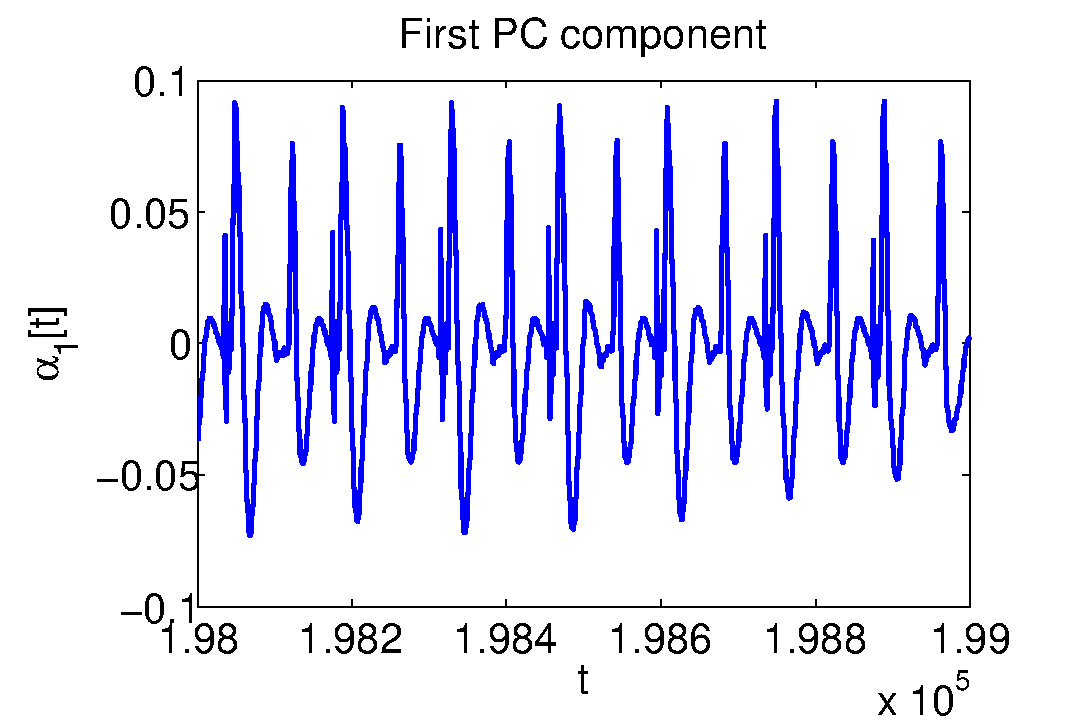
\includegraphics[width=.45\textwidth]{figures/DPAcontestPC1.pdf} 
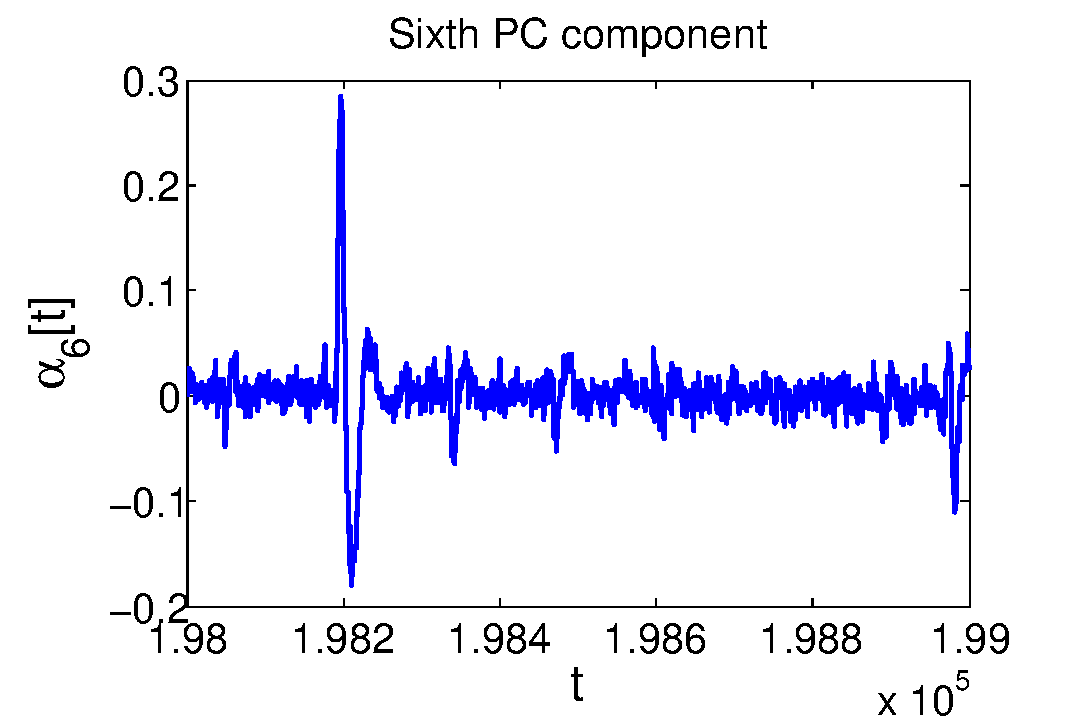
\includegraphics[width=.45\textwidth]{figures/DPAcontestPC6.pdf} 
\caption{First and sixth PCs in DPA contest v4 trace set}\label{fig:DPAcontest}
\end{figure}
To the best of our knowledge, until now only one method adapted to SCA context has been proposed to automatically chose PCs \cite{SCAclassProbl} while dealing with the issue raised in Fig.~\ref{fig:DPAcontest}. It is based on the following assumption:
\begin{assumption}\label{assum:local}
The leaking side-channel information is localised in few points of the acquired trace.
\end{assumption}
In the rest of the paper, we conduct our own analyses under Assumption \ref{assum:local} that we think to be reasonable in SCA contexts where the goal of the security developers is to minimize the number of leaking points.
Under this assumption, the authors of \cite{SCAclassProbl} propose a measure to evaluate the eigenvectors {\em localization}. It is called {\em Inverse Participation Ratio} (IPR) and is defined as follows:
\begin{equation}
\mathrm{IPR}(\AAlpha_i) = \sum_{t=1}^\traceLength \AAlpha_i[t]^4 \mbox{ .}
\end{equation}
The authors of \cite{SCAclassProbl} suggest to collect the PCs in decreasing order with respect to the IPR score.\\

The selection methods provided by the evaluation of the EGV and of the IPR are somehow complementary: the former is based only on the eigenvalues associated to the PCs and does not consider the form of the PCs themselves; the latter completely discards the information given by the eigenvalues of the PCs, considering only the distribution of their coefficients. One of the contributions of the present paper is to propose a new selection method, that builds a bridge between the EGV and the IPR approaches. As we will argue, our method, based on the so-called {\em Explained Local Variance} does not only lead to the construction of a new selection criterion, but also permits  to modify the PCs, choosing individually the coefficients to keep and those to discard. 

%
\subsection{The Explained Local Variance Selection Method} 

\begin{figure}
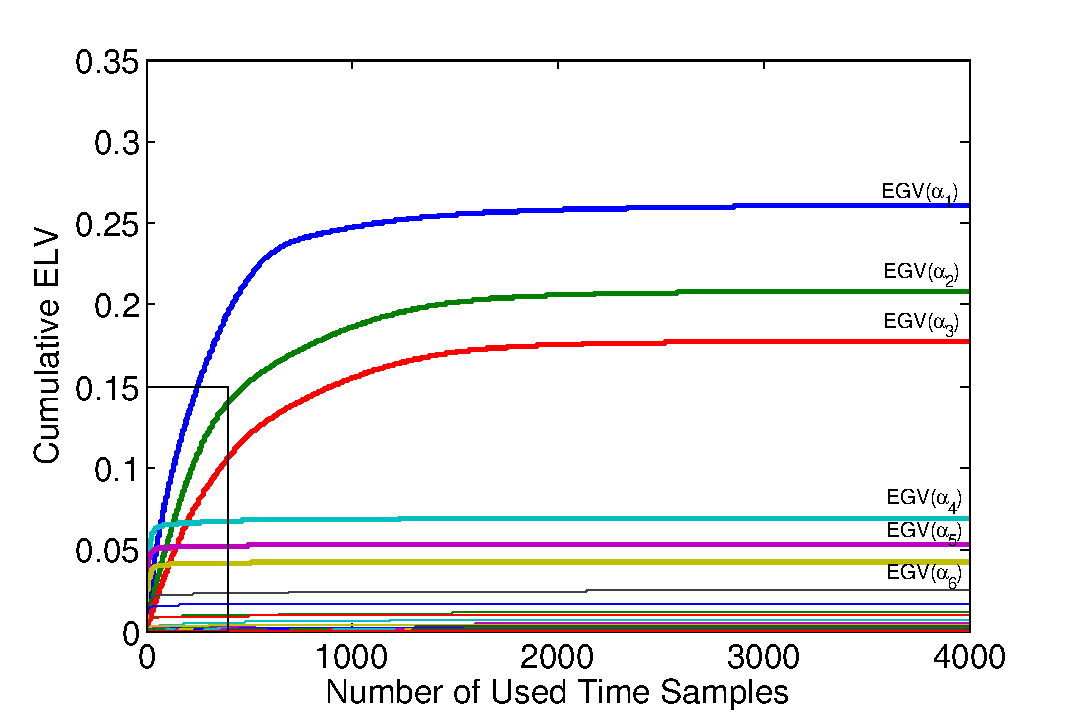
\includegraphics[width=0.5\textwidth]{figures/cumulativeELVallRectangle.pdf} 
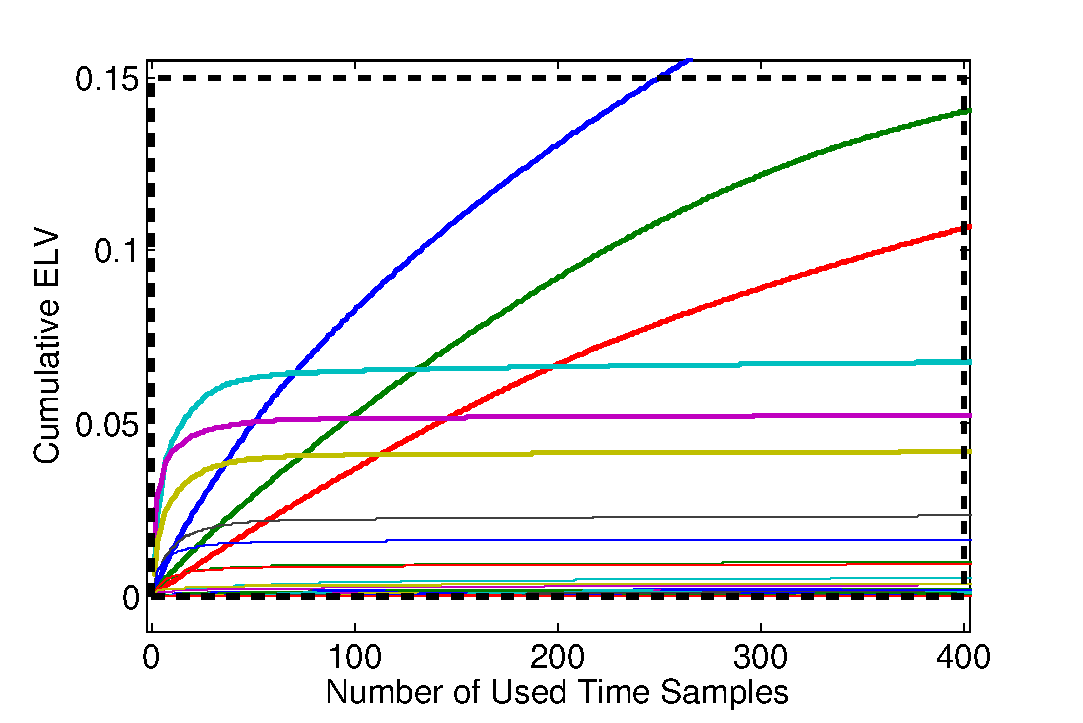
\includegraphics[width=0.5\textwidth]{figures/cumulativeELVzoomedRectangle.pdf} 
\caption{Cumulative ELV trend of principal components. On the right a zoom of the plot on the left. Data acquisition described in Sec.~(\ref{sec:fourCriteria}).}\label{fig:ELVcumulative}
\end{figure}


The method we develop in this section is based on a compromise between the variance provided by each PC (more precisely its EGV) and the number of time samples necessary to achieve a consistent part of such a variance. To this purpose we  introduce the concept of {\em Explained Local Variance} (ELV).\\

Let us start by giving some intuition behind our new concept. Thinking to the observations ${\sss[]{}}^\mathrm{T}$, or to the class-averages ${\mmmX}^\mathrm{T}$ in class-oriented PCA case, as realizations of a random variable $\XXX$, we have that $\lambda_i$ is an estimator for the variance of the random variable $\XXX\cdot\AAlpha_i$. Developing, we obtain
\begin{align}\label{eq:ELV}
\lambda_i =& \hat{\mathrm{var}}(\sum_{j=1}^D \XXX[j]\AAlpha_i[j]) = \sum_{j=1}^D\sum_{k=1}^D \hat{\mathrm{cov}}(\XXX[j]\AAlpha_i[j], \XXX[k]\AAlpha_i[k])=\\
=& \sum_{j=1}^D \AAlpha_i[j]\sum_{k=1}^D\AAlpha_i[k]\hat{\mathrm{cov}}(\XXX[j], \XXX[k])= \sum_{j=1}^D \AAlpha_i[j]\cdot \covmat_{j} \AAlpha_i=  \\
=& \sum_{j=1}^D \AAlpha_i[j]\cdot \lambda_i\AAlpha_i[j]= \sum_{j=1}^D  \lambda_i \AAlpha_i[j]^2 \label{eq:toJustify}
\end{align}
where $\covmat_{j}$ denotes the $j$-th row of $\covmat$ and \eqref{eq:toJustify} is justified by the fact that $\AAlpha_i$ is an eigenvector of $\covmat$, with $\lambda_i$ its corresponding eigenvalue. The result of this computation is quite obvious, since $\parallel \AAlpha_i\parallel=1$, but it evidences the contribution of each time sample in the information held by the PC. This makes us introduce the following definition:
\begin{definition}
The {\em Explained Local Variance} of a PC $\AAlpha_i$ in a sample $j$, is defined by
\begin{equation}
\mathrm{ELV}(i,t) = \frac{\lambda_i \AAlpha_i[t]^2}{\sum_{j=1}^r\lambda_j} = \mathrm{EGV}(i) \AAlpha_i[t]^2  \mbox{ .}
\end{equation}
\end{definition}
\begin{figure}
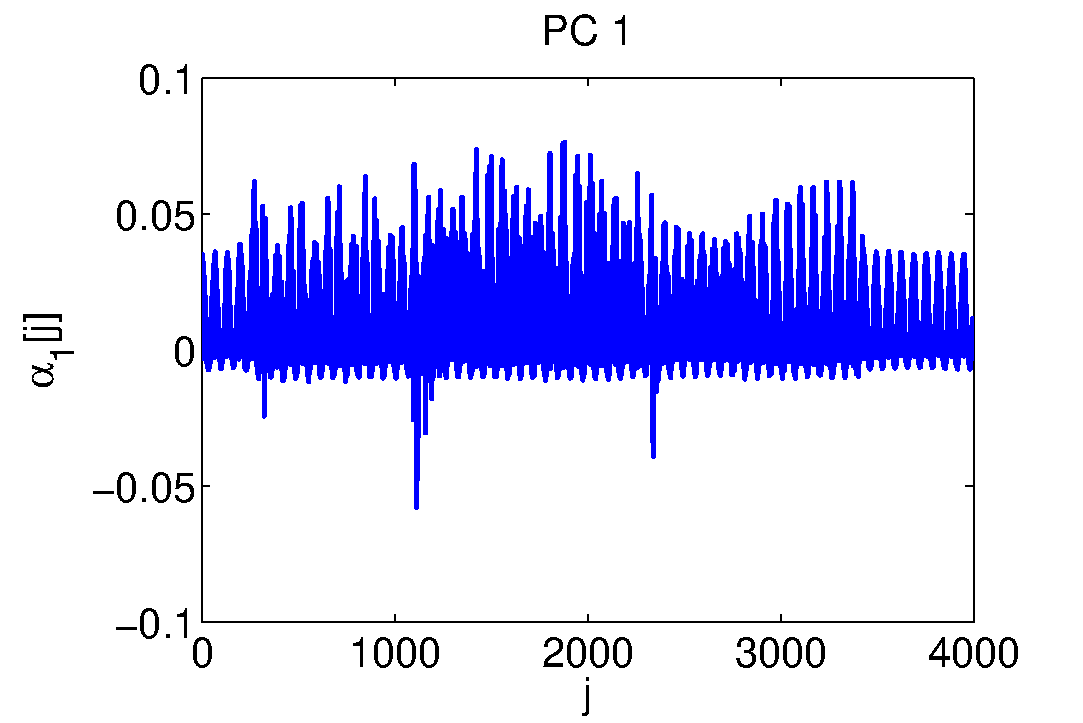
\includegraphics[width=0.31\textwidth]{figures/PC1.pdf} 
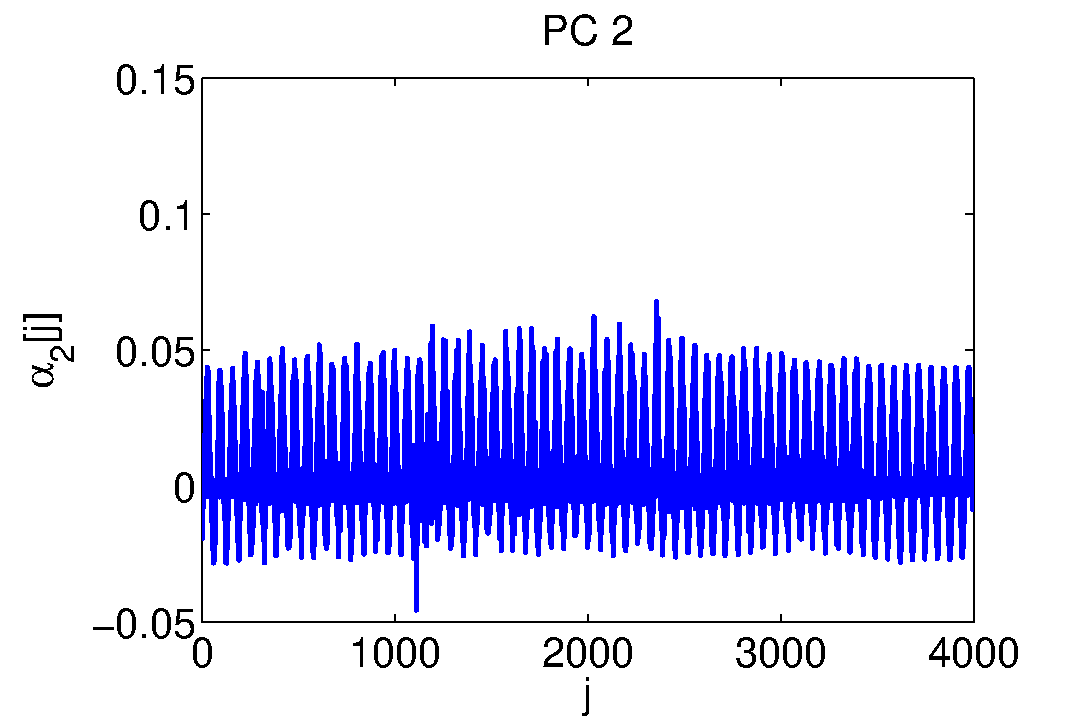
\includegraphics[width=0.31\textwidth]{figures/PC2.pdf} 
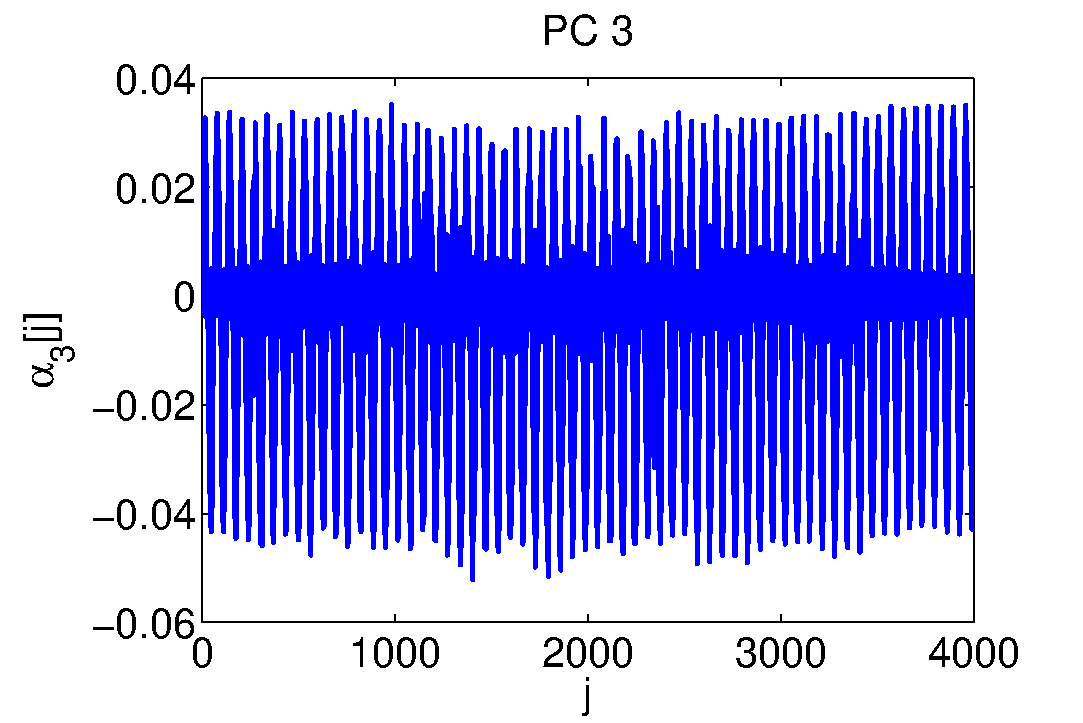
\includegraphics[width=0.31\textwidth]{figures/PC3.pdf} \\
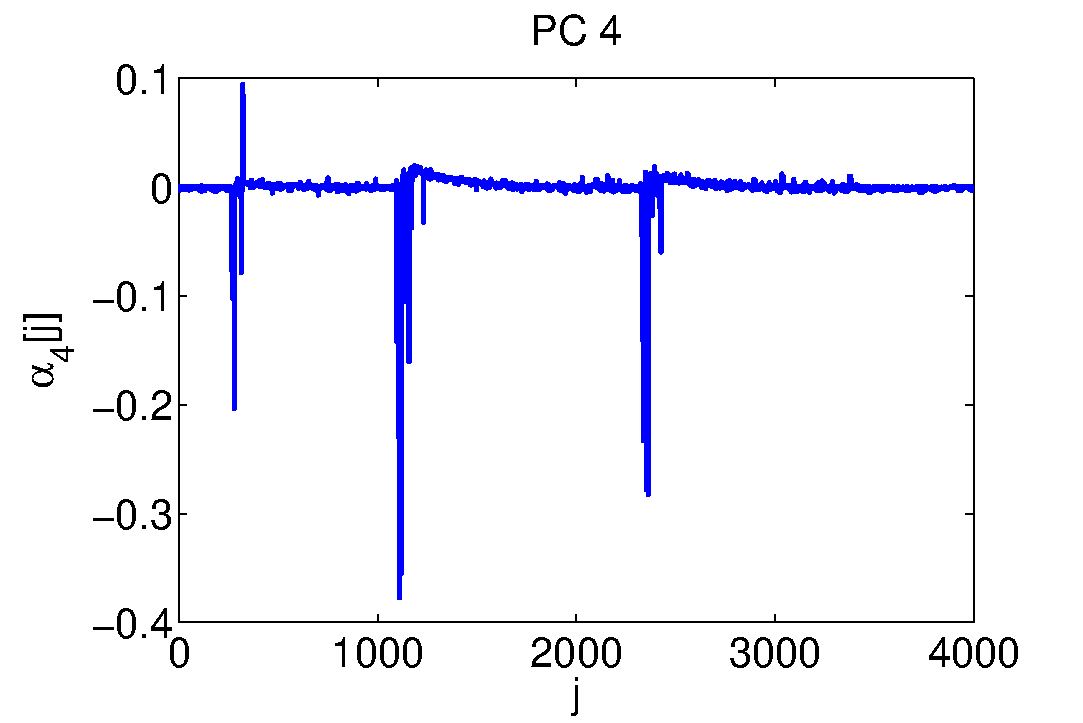
\includegraphics[width=0.31\textwidth]{figures/PC4.pdf} 
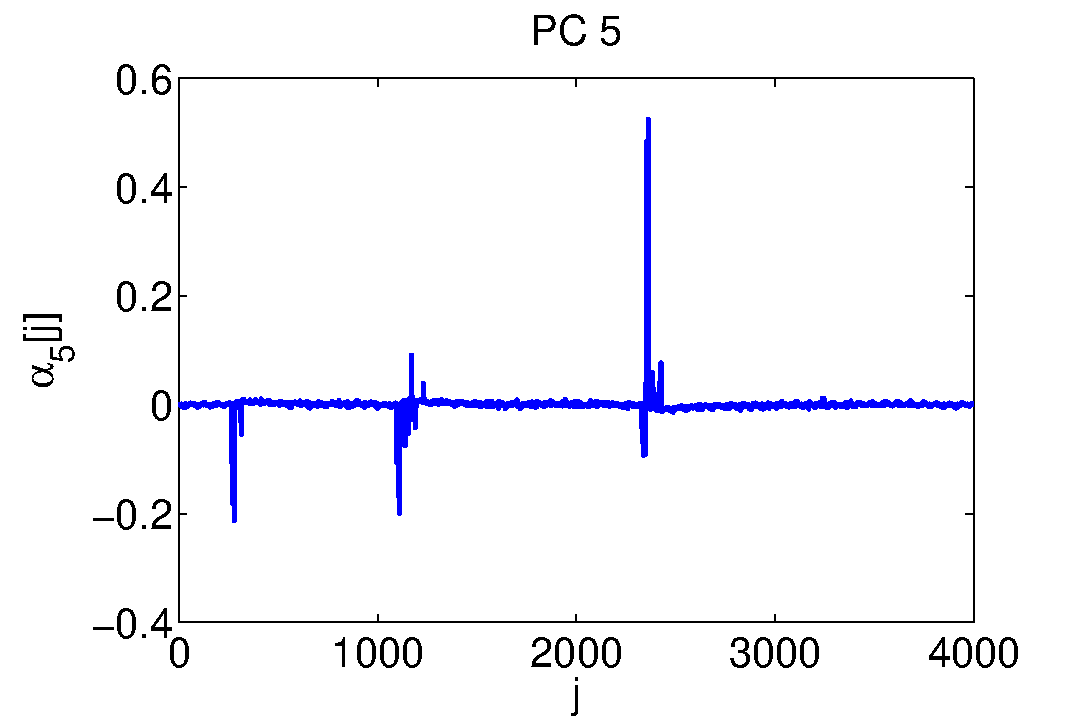
\includegraphics[width=0.31\textwidth]{figures/PC5.pdf} 
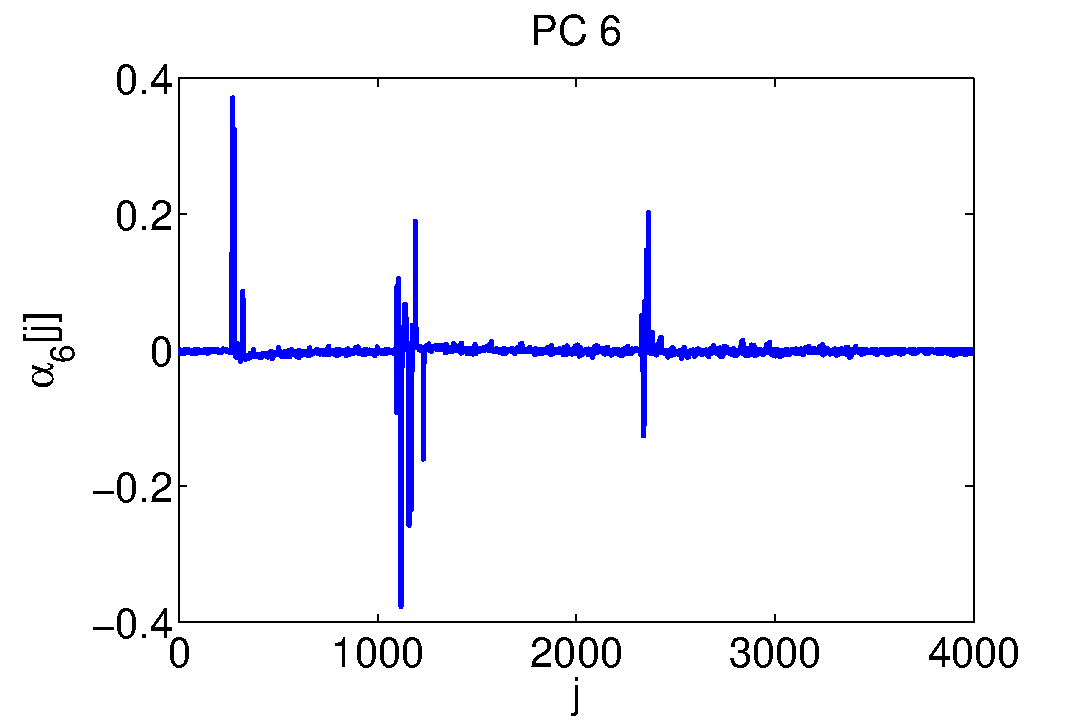
\includegraphics[width=0.31\textwidth]{figures/PC6.pdf} 
\caption{The first six PCs. Acquisition campaign on an 8-bit AVR Atmega328P (see Sec.~\ref{sec:experiments}).}\label{fig:6components}
\end{figure}
It may be observed that the sum over all the trace samples ELVs of a PC equals the EGV of the considered PC. If we operate such a sum for each PC in a cumulative way and in decreasing order over the coefficients starting from the one that holds the maximal ELV, we obtain a complete description of the trend followed by each component to achieve its EGV. As we can see in Fig.~\ref{fig:ELVcumulative}, where such cumulative ELVs are represented, the first 3 components are much slower in achieving their final EGV, while the $4^\text{th}$, the $5^\text{th}$ and the $6^\text{th}$ achieve a large part of their final EGVs very quickly ({\em i.e.} by adding the ELV contributions of much less time samples). This implies that the EGV of the $4^\text{th}$, the $5^\text{th}$ and the $6^\text{th}$ only essentially depends on a very few time samples. This observation, combined with Assumption \ref{assum:local}, suggests that they are more suitable for SCA than the three first ones. To validate this statement, it suffices to look at the form of such components (Fig.~\ref{fig:6components}): the leading ones are very influenced by the clock, while the latest ones are well localised over the leaking points.\\

Operating a selection of components {\em via} ELV, in analogy with the EGV, requires to fix the reduced space dimension $\newTraceLength$, or a threshold $\beta$ for the cumulative ELV. In the first case, the maximal ELVs of each PC are compared, and the $\newTraceLength$ components achieving the highest values of such ELVs are chosen. In the second case, all couples (PC, time sample) are sorted in decreasing order with respect to their ELV, and summed until the threshold $\beta$ is achieved. Then only PCs contributing in this sum are selected. \\

We remark that the ELV is a score associated not only to the whole components, but to each of their coefficients. This interesting property can be exploited to further select, within a selected PC, the non-significant points, {\em i.e.} those with a low ELV, to be setted to zero. That is a natural way to exploit the ELV score in order to operate a kind of {\em denoising} for the reduced data, making them only depend  on the significant time samples. In Sec.~\ref{sec:experiments} we test the performances of an attack varying the number of time samples involved in the computation of the reduced data, and showing that such a denoising processing might impact significantly. 
 


%Actually, the ELV selection method, in analogy with the EGV one, consists in fixing a threshold value $\beta$ for the wished {\em Cumulative Explained Local Variance} and in constructing the set 
%\begin{equation}
%S = \{(i_1, t_1), \dots , (i_{\newTraceLength},t_{\newTraceLength})\} 
%\end{equation}
%where $\newTraceLength$ is the minimal integer such that
%\begin{equation}
%\mathrm{ELV}(i_1,t_1)+\dots +  \mathrm{ELV}(i_{\newTraceLength},t_{\newTraceLength})\geq \beta \mbox{ .}
%\end{equation}
%The rule to choose PCs to keep is then
%\begin{equation}
%\mbox{Keep } \AAlpha_i \Leftrightarrow \exists t \mbox{ such that } (i,t)\in S \mbox{; }
%\end{equation}
%moreover, we propose to only consider, among time samples of each chosen PC, those that hold a significant ELV. For this reason we suggest to consider new PCs $\tilde{\AAlpha}_i$, that we believe incorporate less noise, constructed as follows:
%
%\begin{equation}
%\tilde{\AAlpha}_i[t] = \begin{cases}
%\AAlpha_i[j] \mbox{ if } (i,t)\in S\\
%0 \mbox{ otherwise.}
%\end{cases}
%\end{equation}



%Moreover we define the {\em ELV vector} of a PC $\AAlpha_k$ as the vector $\vectorContribution = (\mathrm{ELV}(k,i))_{i=1..\traceLength}$.
%\end{definition}
%
%
%\subsubsection{{\em Cumulative Explained Local Variance} selection method}
%In this section we present how to select the most informative PCs and how to modify them in order to meaningfully obtain interesting PVs for side channels context.\\
%
%Let $r$ be the rank of the covariance matrix $\covmat$, i.e. the total number of PCs, $\AAlpha_1, \dots, \AAlpha_r$.\\
%Let $\coupleSet = \{1,\dots, r\}\times \{1,\dots,\traceLength\}$ and let us introduce a succession of index couples as
%
%\begin{equation}
%\begin{cases}
%(k_1, i_1) = \mathrm{argmax_{(k,i)\in \coupleSet}}\mathrm{ELV}(k,i)\\
%(k_j, i_j) = \mathrm{argmax_{(k,i)\in \coupleSet\smallsetminus \{(k_1,i_1),\dots,(k_{j-1}, i_{i-1})\}}}\mathrm{ELV}(k,i)\mbox{ .}
%\end{cases}
%\end{equation}
%
%Now fix 
%
%\begin{remark}
%Let $A$ be the matrix that contains the chosen $\tilde{\AAlpha}_k$ vectors as columns. The total variance $\sum diag(A^T\covmat A)$ will not attend the  $\beta$-th part of the initial variables variance, as it would be if eigenvectors $\AAlpha_k$ would have been kept unchanged, but will be lower than it. This is exactly because  vectors $\tilde{\AAlpha}_k$ are no more eigenvectors of $\covmat$. 
%\end{remark}
%
%
%\paragraph{A practical problem that might occur: linear dependent projected data}
%Since the proposed method suggests changing the PCs into new projecting vectors $\tilde{\AAlpha}_k$, the property of decorrelating principal variables is lost. On the contrary it might happen, especially if some $\tilde{\AAlpha}_k$ have only a few non-zero coefficients, that data are projected into new  perfectly correlated coordinates. That is a problem if, for example, the projected data are intended to be used to construct templates for a template attack: the covariance matrix of a random vector with two or more perfectly correlated components is singular, thus, non-invertible, and if templates have non-invertible covariance matrices the template attack is impracticable. \\
%Let $A = [\AAlpha_1, \dots , \AAlpha_\newTraceLength]$ be the matrix containing as columns the projecting components chosen via \emph{Cumulative ELV method}. The problem just described arises whenever such components present a linear dependency, i.e. the matrix $A$ has not maximal rank. This means that one or more components just create new projected variables that are linear combinations of variables constructed by the other components. In practice one or more components do not add any information, and their suppression would not cause an effective lost of \emph{ELV}. That is why as a last passage of our method we propose to check that the projecting matrix has maximal rank $\newTraceLength$, and, if it has not, suppress from it the minimal number of columns that makes it attend its maximal rank. 
%
%
%
%

\section{Linear Discriminant Analysis}\label{sec:LDA}

Linear Discriminant Analysis (LDA) is another statistical tool for dimensionality reduction, which is theoretically more appropriate than PCA for classification problems as SCA, as already observed in \cite{Standaert2008}. Indeed it seeks for linear combinations of data that characterize or separate two or more classes, not only spreading class centroids as much as possible, like the class-oriented PCA does, but also minimizing the so-called {\em intra-class variance}, i.e. the variance shown by data belonging to the same class.\\

\subsubsection{Description.} Applying LDA consists in maximizing the so-called {\em Rayleigh quotient}:
 \begin{equation}\label{eq:LDA}
 \AAlpha_1=\mathrm{argmax}_{\AAlpha} \frac{\AAlpha^T \SB \AAlpha}{\AAlpha^T \SW \AAlpha} \mbox{ ,}
 \end{equation}
where $\SB$ is the {\em between-class scatter matrix} already defined in \eqref{eq:SB} and $\SW$ is called 
{\em within-class} (or intra-class) {\em scatter matrix}:

\begin{equation}
\SW = \sum_{\sensVar\in\sensVarSet}\sum_{i=1}^{\numTraces}(\sss{i}-\mmmX)(\sss{i}-\mmmX)^T \mbox{.}
\end{equation}


\begin{remark}
Let $\covmat$ be the the global covariance matrix of data, also called {\em total scatter matrix}, defined in \eqref{eq:covmat}; we have the following relationship between $\SW,\SB$ and $\covmat$:
\begin{equation}
\covmat = \frac{1}{\numTraces[]}(\SW + \SB) \mbox{ .}
\end{equation}
\end{remark}

It can be shown that the vector $\AAlpha_1$ which maximizes \eqref{eq:LDA} must satisfy $\SB\AAlpha_1 = \lambda \SW \AAlpha_1$, for a constant $\lambda$, \textit{i.e.} has to be an eigenvector of $\SW^{-1} \SB$. Moreover, for any eigenvector $\AAlpha$ of $\SW^{-1}\SB$, with associated eigenvalue $\lambda$, the Rayleigh quotient equals such a $\lambda$:
\begin{equation}\label{eq:lambdas}
\frac{\AAlpha^T \SB \AAlpha}{\AAlpha^T \SW \AAlpha} = \lambda \mbox{ .}
\end{equation}
Then, among all eigenvectors $\SW^{-1} \SB$, $\AAlpha_1$ must be the leading one.\\

The computation of the eigenvectors of $\SW^{-1} \SB$ is known under the name of {\em generalized eigenvector problem}. The difficulty here comes from the fact that $\SW^{-1} \SB$ is not guaranteed to be symmetric. Due to this non-symmetry,  $\AAlpha_1$ and the others eigenvectors do not form an orthonormal basis for $\mathbb{R}^\traceLength$, but they are anyway useful for classifications scopes, as in SCA. Let us refer to them as {\em Linear Discriminant Components} (LDCs for short); as for PCs we consider them sorted in decreasing order with respect to their associated eigenvalue, which gives a score for their informativeness, see \eqref{eq:lambdas}. Analogously to the PCA, the LDA provides a natural dimensionality reduction: one can project the data over the first $\newTraceLength$ LDCs. As for PCA, this choice might not be optimal when applying this reduction to side-channel traces. For the sake of comparison, all the selection methods proposed for the PCA (EGV, IPR and ELV) will be tested in association to the LDA as well.\\

In the following subsection we will present a well-known problem that affects the LDA in many practical contexts, and describe four methods that circumvent such a problem, with the intention to test them over side-channel data.



\subsection{The Small Sample Size Problem}\label{sec:SSS}
In the special case in which the matrix $\SB$ is invertible, the generalized eigenvalue problem is convertible in a regular one, as in \cite{Standaert2008}. On the contrary, when $\SB$ is singular, the simultaneous diagonalization is suggested to solve such a problem \cite{Fukunaga}. In this case one can take advantage by the singularity of $\SB$ to apply the computational trick proposed by Archambeau \textit{et al.}, see Sec.~(\ref{sec:PCA_classes}), since at most $r = \mathrm{rank}(\SB)$ eigenvectors can be found.\\

If the singularity of $\SB$ does not affect the LDA dimensionality reduction, we cannot say the same about the singularity of $\SW$:  SCA and Pattern Recognition literature, points out the same drawback of the LDA, which is known as the {\em Small Sample Size problem} (SSS for short). It occurs when the total number of acquisitions $\numTraces[]$ is less than or equal to the size $\traceLength$ of them.\footnote{It can happen for example when attacking an RSA implementation, where the acquisitions are often huge (of the order of 1,000,000 points) and the number of measurements may be small when the SNR is good, implying that a good GE can be achieved with a small $N$.} The direct consequence of this problem is the singularity of $\SW$ and the non-applicability of the LDA. \\

If the LDA has seen introduced relatively lately in the SCA literature, the Pattern Recognition community looks for a solution to the SSS problem at least since the early nineties. We browsed some of the proposed solution and chose some of them to introduce, in order to test them over side channel traces.

\subsubsection{Fisherface Method}
The most popular among the solutions to SSS is the so-called {\em Fisherface} method\footnote{The name is due to the fact that it was proposed and tested for face recognition scopes.} \cite{eigenfaces}. It simply relies on the combination between PCA and LDA: a standard PCA dimensionality reduction is performed to data, making them pass from dimension $\traceLength$ to dimension $\numTraces[]-\lvert \sensVarSet \rvert$, which is the general maximal rank for $\SW$. In this reduced space, $\SW$ is very likely to be invertible and the LDA therefore applies.

\subsubsection{$SW$ Null Space Method}
It has been introduced by Chen {\em et al.} in \cite{Chen2000} and exploits an important result of Liu {\em et al.} \cite{liu1992generalized} who showed that Fisher's criterion \eqref{eq:LDA} is equivalent to:
 \begin{equation}
 \AAlpha_1=\mathrm{argmax}_{\AAlpha} \frac{\AAlpha^T \SB \AAlpha}{\AAlpha^T \SW \AAlpha + \AAlpha^T \SB \AAlpha} \mbox{ .}
 \end{equation}
The authors of \cite{Chen2000} point out that such a formula is upper-bounded by 1, and that it achieves its maximal value, \textit{i.e.} 1, if and only if  $\AAlpha$ is in the null space of $\SW$. Thus they propose to first project data onto the null space of $\SW$ and then to perform a PCA, \textit{i.e.} to select as LDCs the first $\lvert \sensVarSet \rvert - 1$ eigenvectors of the between-class scatter matrix of data into this new space. More precisely, let $Q = [\vvv_1, \dots, \vvv_{\traceLength - \mathrm{rank}(\SW)}]$ be the matrix of vectors that span the null space of $\SW$. \cite{Chen2000} proposes to transform the data $\sss[]{}$ into $\xxx' = QQ^T\xxx$. Such a transformation maintains the original dimension $\traceLength$ of the data, but let the new within-class matrix $\SW' = QQ^T\SW QQ^T$ be the null $\traceLength \times \traceLength$ matrix. Afterwards, the method looks for the eigenvectors of the new between-class matrix $\SB' = QQ^T\SB QQ^T$. Let $U$ be the matrix containing its first $\lvert \sensVarSet \rvert - 1$ eigenvectors: the LDCs obtained via the $\SW$ null space method are the columns of $QQ^TU$.

\subsubsection{Direct LDA}
As the previous, this method, introduced in \cite{Yu01adirect} privileges the low-ranked eigenvectors of $\SW$, but proposes to firstly project the data onto the rank space of $\SB$, arguing the fact that vectors of the null space of $\SB$ do not provide any between-class separation of data. \\
Let $D_B=V^T\SB V$ be the singular value decomposition of $\SB$, and let $V^\star$ be the matrix of the eigenvectors of $\SB$ that are not in its null space, \textit{i.e.} whose eigenvalues are different from zero. Let also $D_B^\star$ denotes the matrix ${V^\star}^T\SB V^\star$; transforming the data $\xxx$ into ${D_B^\star}^{1/2}{V^\star}^T\xxx$ makes the between-class variance to be equal to   the $(\lvert \sensVarSet \rvert - 1 \times \lvert \sensVarSet \rvert - 1)$ identity matrix. After this transformation the within-class variance assumes the form $\SW' = {D_B^\star}^{1/2}{V^\star}^T\SW ' V^\star {D_B^\star}^{1/2}$. After storing the $\newTraceLength$ lowest-rank eigenvectors in a matrix $U^\star$, the LDCs obtained via the Direct LDA method are the columns of $V^\star{D_B^\star}^{1/2}{U^\star}^T$. Observe that for the first projection, there is no need to compute the big $\SB$ matrix, because the computational trick of Sec.~\ref{sec:PCA_classes} is applicable.


\subsubsection{$\ST$ Spanned Space Method}
The last variant of LDA that we consider has been proposed in \cite{huang} and is actually a variant of the Direct LDA: instead of removing the null space of $\SB$ as first step, this method removes the null space of $\ST = \SB + \SW$. Then, denoting $\SW'$ the within-class matrix in the reduced space, the reduced data are projected onto its null space, i.e. are multiplied by the matrix storing by columns the eigenvectors of $\SW'$ associated to the null eigenvector, thus reduced again. A final optional step consists in verifying if  the between-class matrix presents a non-trivial null-space after the last projection and, in this case, in effectuating a further projection removing it.





\section{Experimental Results}\label{sec:experiments}

In this section we compare the different extractors provided by the PCA and the LDA in association with the different techniques  of components selection. Defining an optimal extractor  is not a trivial task, especially because a universal criterion to compare different extractors must encompass a lot of parameters that vary according to the context (amount of noise, specificity of the information leakage, nature of the side channel, etc.). For this reason we will focus on a given adversary, and specify four different goals that may be pursued by the attacker: 
\begin{enumerate}
\item {\em Minimize $\numTraces[]$}: achieve $\guessingEntropy_{\adversary'}\leq \threshold$ with the minimal number of attack traces, with $\threshold$ a fixed threshold, common to the four goals
\item {\em Minimize $\numTraces[]'$}: achieve $\guessingEntropy_{\adversary'}\leq \threshold$ with the minimal number of profiling traces
\item {\em Minimize $\newTraceLength$}: achieve $\guessingEntropy_{\adversary'}\leq \threshold$ reducing as much as possible the size of the extracted traces
\item {\em Minimize $\numPoI$}: achieve $\guessingEntropy_{\adversary'}\leq \threshold$ exploiting the minimal number of original trace points.
\end{enumerate}
 
 To compare the techniques discussed in this paper, we will refer to the four goal above, considering four scenarios: in each one, three of the four parameters $\numTraces[], \numTraces[]', \newTraceLength, \numPoI$ are fixed and one varies. For those in which $\numTraces[]'$ is fixed, the value of $\numTraces[]'$ is chosen high enough to avoid the SSS problem, and the extensions of LDA presented in Sec.~\ref{sec:SSS} are not evaluated.\footnote{This study is let open for an extended version of this paper.} This choice of $\numTraces[]'$ will imply that the LDA is always performed in a favourable situation, which makes expect the LDA to be particularly efficient for these experiments. Consequentely, for the scenarios in which $\numTraces[]'$ is high, our goal is to study whether the PCA can be made almost as efficient as the LDA thanks to the component selection methods discussed in Sec.~\ref{sec:ELV}. 



\subsubsection{The testing adversary.}  Our testing adversary attacks an 8-bit AVR microprocessor Atmega328P and acquires power-consumption traces via the ChipWhisperer platform \cite{o2014chipwhisperer}.\footnote{This choice has been done, in particular, to allow for reproducibility of the experiments.} The target device stores a secret 128-bit key and performs the first steps of an AES: the loading of 16 bytes of the plaintext, the AddRoundKey step and the AES Sbox. It has been programmed twice: two different keys are stored in the device memory during the acquisition of the profiling and of the attack traces, to simulate the situation of two identical devices storing a different secret. The size $\traceLength$ of the traces equals $3996$. The sensitive target  variable is the output of the first Sbox processing, but, since the key is fixed also during the profiling phase, and both Xor and Sbox operations are bijective, we expect to detect three interesting regions (as those high-lighted by PCs 4, 5 and 6, in Fig.~\ref{fig:6components}): the reading of the first byte of the plaintext, the first AddRoundKey and the first Sbox. We consider an {\em identity classification} leaking function (i.e. we make minimal assumption on the leakage function), which implies that the 256 possible values of the Sbox output yields to 256 classes. For each class we assume that the adversary acquires the same number $N_p$ of traces, \textit{i.e.} $\numTraces[]' = N_p\times 256$. After the application of the extractor $\extract$, the trace size is reduced to $\newTraceLength$. Then the attacker performs a Bayesian Template Attack \cite{Chari2003}, using $\newTraceLength$-variate Gaussian templates. This choice comes from the information-theoretic optimality of such an attack which, exploiting the maximum likelihood parameters estimation, yields to an unbiased comparison between the extractors.


\subsubsection{Scenario 1.}
To analyse the dependence between the extraction methods presented in Sections ~\ref{sec:PCA} and \ref{sec:LDA} and the number of attack traces $\numTraces[]$ needed to achieve a given GE, we fixed the other parameters as follows: $N_p=50$ ($\numTraces[]'=50*256$), $\newTraceLength = 3$ and $\numPoI = 3996$ (all points are allowed to participate in the building of the PCs and of the LDCs). The experimental results, depicted in Fig.~\ref{fig:1and2} \subref{fig:1.1}-\subref{fig:1.2}, show that the PCA standard method has very bad performances in SCA, while the LDA outperforms the others. Concerning the class-oriented PCA, we observe that its performance is comparable to that of LDA when combined with the selection methods ELV (which performs best) or IPR.  



\subsubsection{Scenario 2.}
%\begin{figure}
%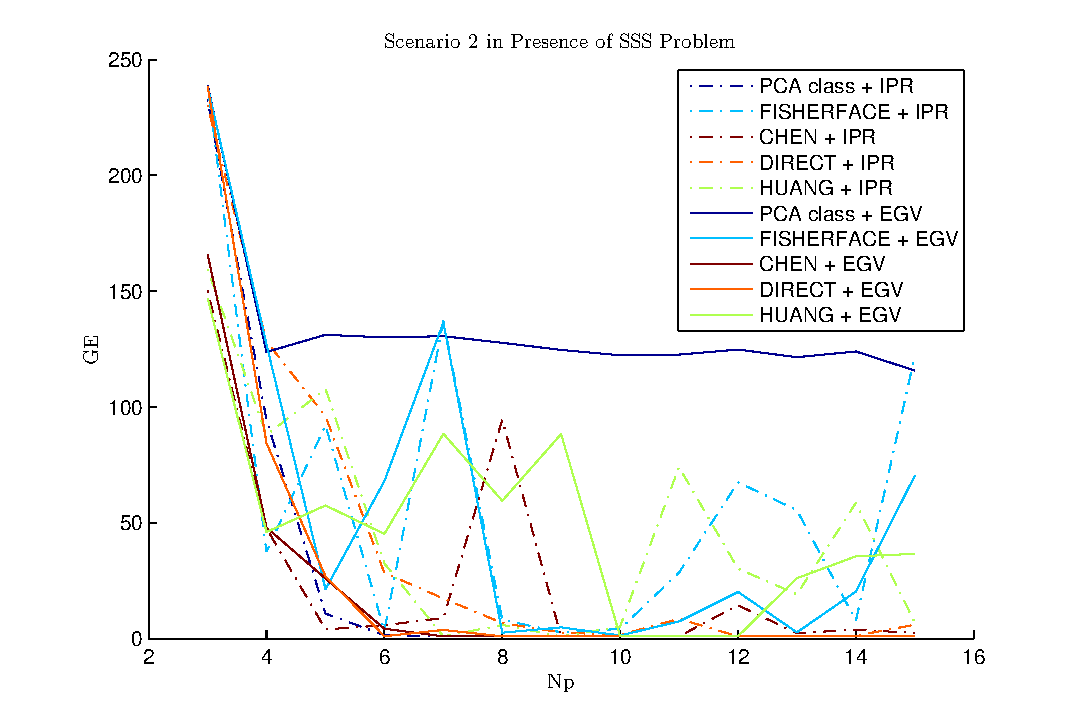
\includegraphics[width=0.5\textwidth]{figures/Criterion2SSS.pdf}
%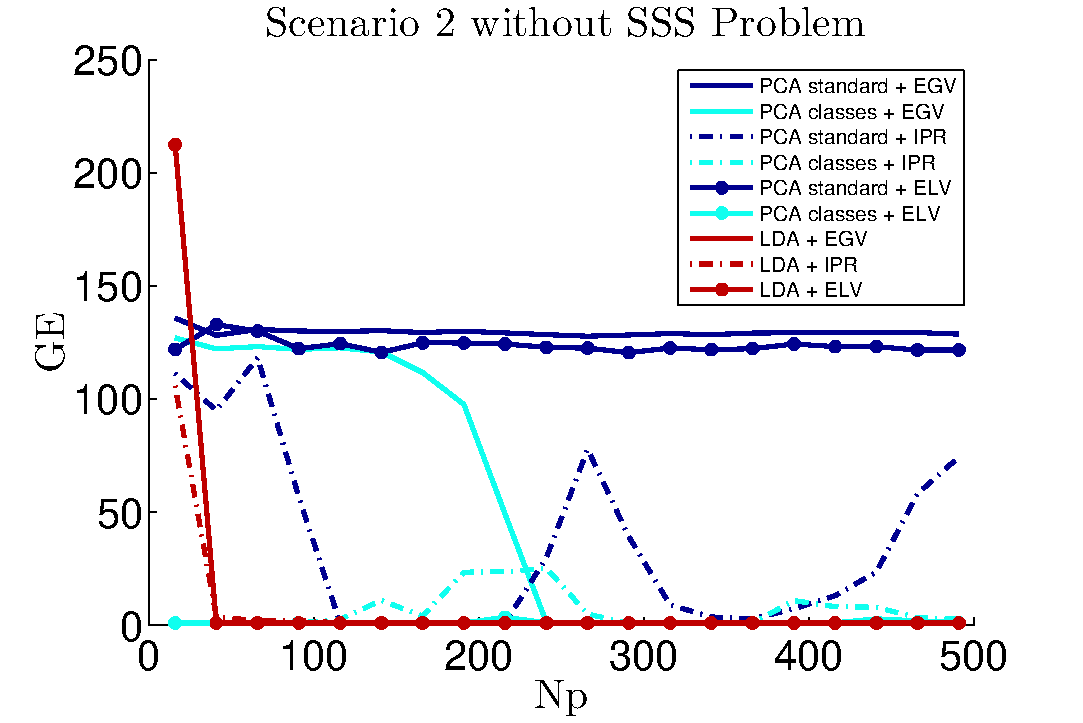
\includegraphics[width=0.5\textwidth]{figures/Criterion2notSSS.pdf} 
%\caption{Guessing Entropy as function of the number of profiling traces per class, for different extraction methods: on the left the LDA is substituted by its extensions to handle the SSS problem.}\label{fig:2}
%\end{figure}
Now we test the behaviour of the extraction methods as function of the number $N_p$ of available profiling traces per class. The number of components $\newTraceLength$ is still fixed to 3, and $\numPoI=3996$ again. This scenario has to be divided into two parts: if $N_p\leq 15$, then $\numTraces[]'<\traceLength$ and the SSS problem occurs. Thus, in this case we will test the four extensions of LDA presented in Sec.~\ref{sec:SSS}, associated to either the standard selection, to which we abusively refer as EGV,\footnote{It consists in keeping the $\newTraceLength$ first LDCs, except for the Direct LDA, which asks to keep the last LDCs.} and to the IPR selection.  We compare them to the class-oriented PCA associated to EGV, IPR and ELV. The ELV selection is not performed for the techniques extending LDA, since for some of them the projecting LDCs are not associated to some eigenvalues in a meaningful way. On the contrary, if $N_p\geq 16$ there is no need to approximate the LDA technique, so the classical one is performed. Results for this scenario are shown in Fig.~\ref{fig:1and2} \subref{fig:2.1}-\subref{fig:2.2}. It may be noticed that the combinations class-oriented PCA + ELV/IPR (that select exactly the same components, for our data) do not suffer from the lack of profiling traces. They are slightly outperformed by the Chen method in association to EGV. The Direct LDA method also provides a good alternative, while the other tested methods do not show a stable behaviour. The results in absence of the SSS problem confirm that the standard PCA is not adapted to SCA, even when provided with more profiling traces. It also shows that among class-oriented PCA and LDA, the class-oriented PCA converges faster.

\begin{figure}[h!]
\subfigure[]{\label{fig:1.1}
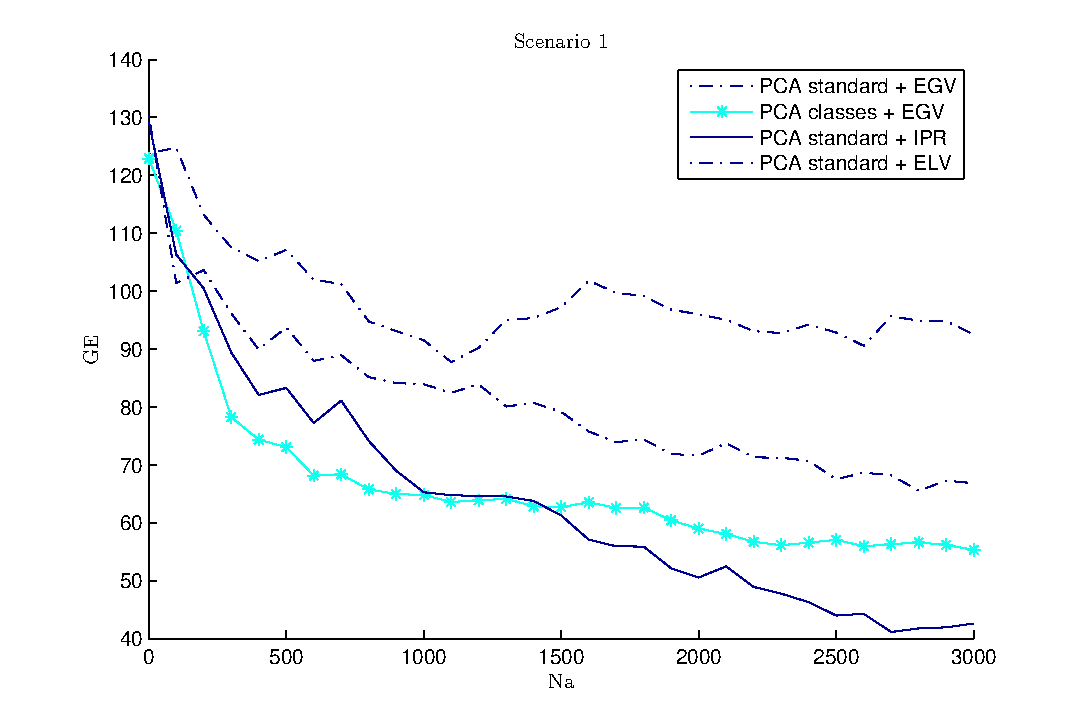
\includegraphics[width=0.5\textwidth]{figures/Criterion1.pdf}}
\subfigure[]{\label{fig:1.2}
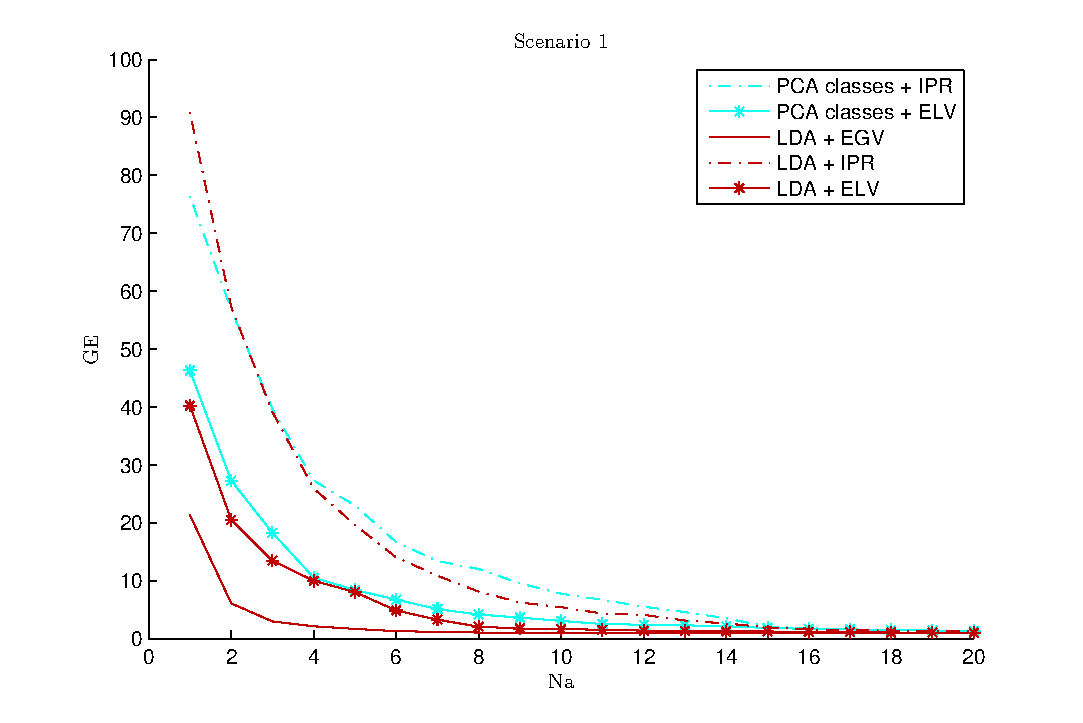
\includegraphics[width=0.5\textwidth]{figures/Criterion1Good.pdf}}
\subfigure[]{\label{fig:2.1}
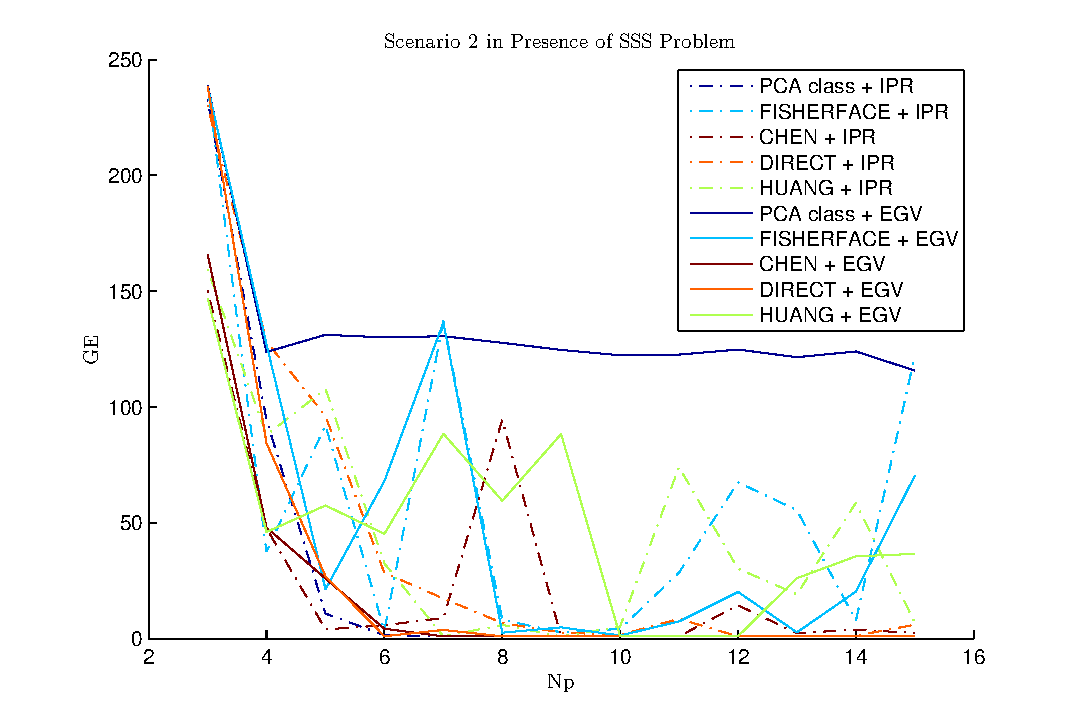
\includegraphics[width=0.5\textwidth]{figures/Criterion2SSS.pdf}}
\subfigure[]{\label{fig:2.2}
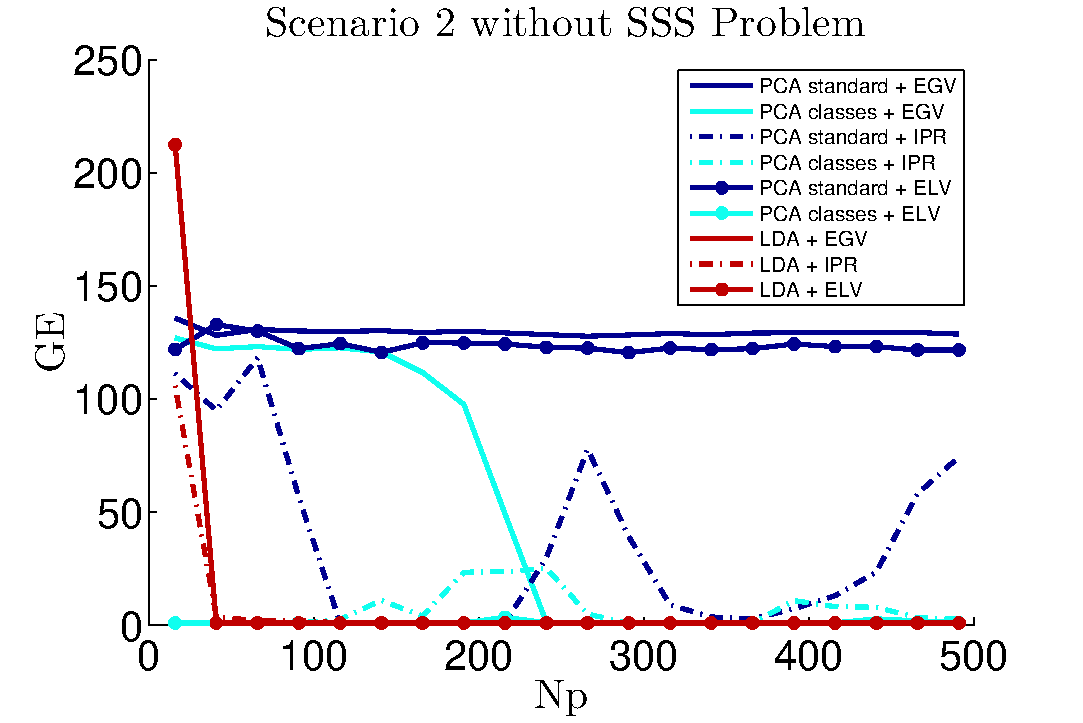
\includegraphics[width=0.5\textwidth]{figures/Criterion2notSSS.pdf}}
\caption{Guessing Entropy as function of the number of attack traces \ref{fig:1.1},\ref{fig:1.2} and of the number of profiling traces per class \ref{fig:2.1}, \ref{fig:2.2}, for different extraction methods. In \ref{fig:2.1} the LDA is substituted by its extensions to handle the SSS problem. All Guessing Entropies are estimated as the average rank of the right key over 100 independent experiments.}\label{fig:1and2}
\end{figure}

\subsubsection{Scenario 3.}
Let  $\newTraceLength$ be now variable and let the other parameters be fixed as follows: $\numTraces[] = 100, N_p=200, \numPoI = 3996$. Looking at Fig.~\ref{fig:3}, we might observe that the standard PCA might actually well perform in SCA context if provided with a larger number of kept components; on the contrary, a little number of components suffices to the LDA. Finally, keeping more of the necessary components does not worsen the efficiency of the attack, which allows the attacker to choose $\newTraceLength$ as the maximum value supported by his computational means.

\begin{remark}
In our experiments the ELV selection method only slightly outperforms the IPR. Nevertheless, since it relies on more sound and more general observations, {\em i.e.} the maximization of explained variance concentrated into few points, it is likely to be more robust and less case-specific.
\end{remark}


\subsubsection{Scenario 4.}


This is the single scenario in which we allow the ELV selection method to not only select the components to keep but also to modify them, keeping only some coefficients within each component, setting the other ones to zero. We select pairs \textit{(component, time sample)} in decreasing order of the ELV values, allowing the presence of only $\newTraceLength = 3$ components and $\numPoI$ different times samples: {\em i.e.}, we impose that the matrix $A$ defining the extractor (see \eqref{eq:linearExtractor}) has $\newTraceLength = 3$ rows (storing the 3 chosen components, transposed) and exactly $\numPoI$ non-zero columns.
Looking at Fig.~\ref{fig:4} we might observe that the LDA allows to achieve the maximal guessing entropy with only 1 PoI in each of the 3 selected components. 
Actually, adding PoIs worsen its performances, which is coherent with the assumption that the vulnerable information leaks in only a few points. Such points are excellently detected by the LDA. Adding contribution from other points raises the noise, which is then compensated by the contributions of further noisy points, in a very delicate balance. Such a behaviour is clearly visible in standard PCA case: the first 10 points considered raise the level of noise, that is then balanced by the last 1000 points.

\medskip

  \begin{minipage}[c]{\textwidth}
  \hspace*{-3mm}
  \begin{minipage}[c]{0.49\textwidth}
    \centering
    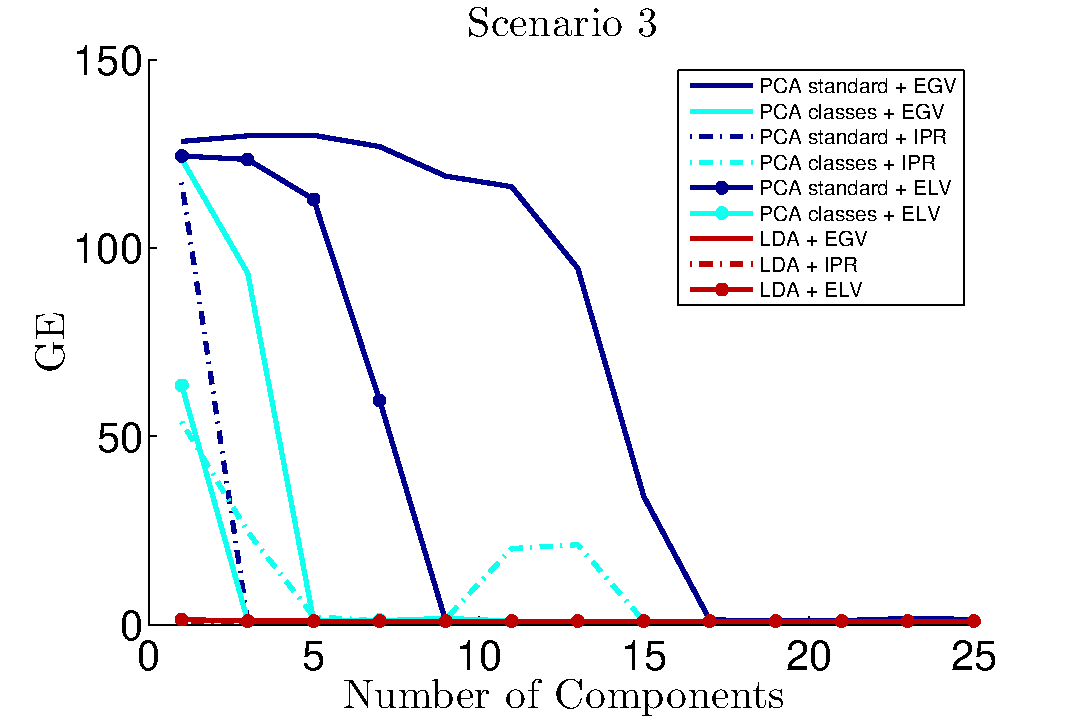
\includegraphics[width=\textwidth]{figures/Criterion3.pdf}
    \captionof{figure}{Guessing Entropy as function of the number of the traces size after reduction}\label{fig:3}
  \end{minipage}
\hspace{1mm}
  \begin{minipage}[c]{0.45\textwidth}
    \centering
    \begin{tiny}
\begin{tabular}{|c|c|c|c|c|c|}
\hline
&&\multicolumn{4}{|>{\columncolor[gray]{0.7}}c|}{Parameter to minimize}\\
\hline
\multicolumn{1}{|>{\columncolor[gray]{0.7}}c|}{Method}&\multicolumn{1}{|>{\columncolor[gray]{0.7}}c|}{Selection}& $N$ &  $N'$ (SSS) &  $N'$ (not SSS) &  $C$ \\
\hline
PCA standard & EGV & {\bf -} &  &{\bf -} &{\bf -} \\
\hline
PCA standard &\multicolumn{1}{|>{\columncolor[gray]{0.8}}c|}{ELV} & \multicolumn{1}{|>{\columncolor[gray]{0.9}}c|}{{\bf -}} & &\multicolumn{1}{|>{\columncolor[gray]{0.9}}c|}{{\bf -}} &\multicolumn{1}{|>{\columncolor[gray]{0.9}}c|}{{\bf -}} \\
\hline
PCA standard & IPR &{\bf -} & &{\bf -} &{\bf +} \\
\hline
PCA class & EGV & {\bf -} &{\bf -} &{\bf -} &{\bf -} \\
\hline
PCA class & \multicolumn{1}{|>{\columncolor[gray]{0.8}}c|}{ELV} &\multicolumn{1}{|>{\columncolor[gray]{0.9}}c|}{{\bf +}} &\multicolumn{1}{|>{\columncolor[gray]{0.9}}c|}{$\bigstar$}&\multicolumn{1}{|>{\columncolor[gray]{0.9}}c|}{$\bigstar$} &\multicolumn{1}{|>{\columncolor[gray]{0.9}}c|}{{\bf +}} \\
\hline 
PCA class & IPR & {\bf {\bf +}} &$\bigstar$ &{\bf +} &{\bf -} \\
\hline 
LDA & EGV &$\bigstar$ & & {\bf +} & $\bigstar$\\
\hline 
LDA & \multicolumn{1}{|>{\columncolor[gray]{0.8}}c|}{ELV} & \multicolumn{1}{|>{\columncolor[gray]{0.9}}c|}{{\bf +}} &  & \multicolumn{1}{|>{\columncolor[gray]{0.9}}c|}{{\bf +}} & \multicolumn{1}{|>{\columncolor[gray]{0.9}}c|}{$\bigstar$}\\
\hline 
LDA & IPR & {\bf +} & &{\bf +} & $\bigstar$ \\

\hline 
\multicolumn{1}{|>{\columncolor[gray]{0.8}}c|}{$\SW$ Null Space}  & EGV & &\multicolumn{1}{|>{\columncolor[gray]{0.9}}c|}{$\bigstar$ } & & \\
\hline 
\multicolumn{1}{|>{\columncolor[gray]{0.8}}c|}{$\SW$ Null Space}  & IPR & &\multicolumn{1}{|>{\columncolor[gray]{0.9}}c|}{{\bf +}} & & \\
\hline 
\multicolumn{1}{|>{\columncolor[gray]{0.8}}c|}{Direct LDA} & EGV & & \multicolumn{1}{|>{\columncolor[gray]{0.9}}c|}{$\bigstar$}& & \\
\hline 
\multicolumn{1}{|>{\columncolor[gray]{0.8}}c|}{Direct LDA} & IPR & &\multicolumn{1}{|>{\columncolor[gray]{0.9}}c|}{{\bf +}}& & \\
\hline
\multicolumn{2}{|>{\columncolor[gray]{0.8}}c|}{Fisherface} & &\multicolumn{1}{|>{\columncolor[gray]{0.9}}c|}{{\bf -}} & & \\
\hline 
\multicolumn{2}{|>{\columncolor[gray]{0.8}}c|}{$\ST$ Spanned Space}  & &\multicolumn{1}{|>{\columncolor[gray]{0.9}}c|}{{\bf -}} & & \\
\hline
\end{tabular}
\end{tiny}
\captionof{table}{Overview of extractors performances in tested situations.}\label{table:results}
    \end{minipage}
  \end{minipage}




\begin{figure}
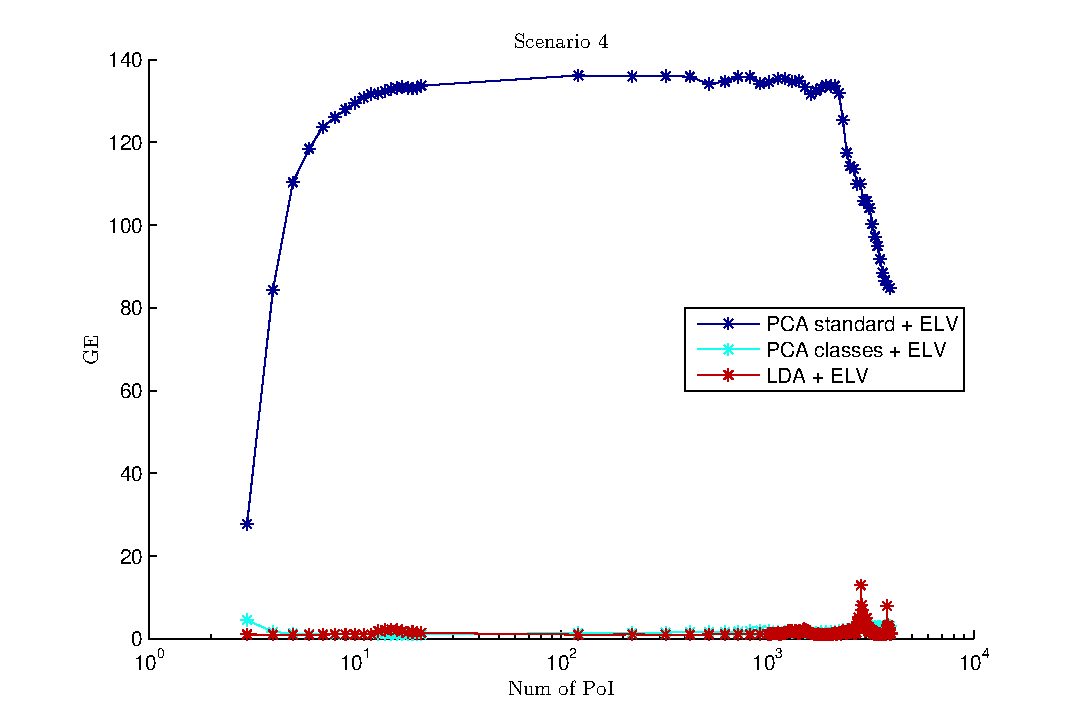
\includegraphics[width=0.5\textwidth]{figures/Criterion4.pdf}
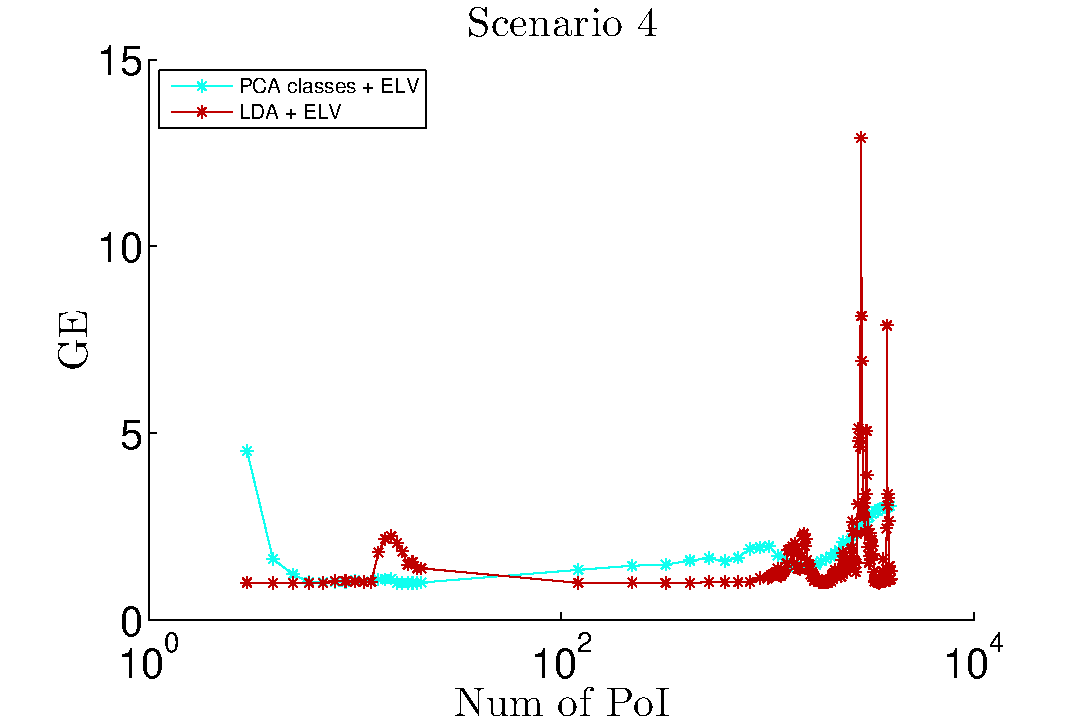
\includegraphics[width=0.5\textwidth]{figures/Criterion4cutted.pdf} 
\caption{Guessing Entropy as function of the number of time samples contributing to the extractor computation.}\label{fig:4}
\end{figure}



\medskip

An overview of the results of our comparison in scenarios 1, 2 and 3 is depicted in Table~\ref{table:results}: depending on the adversary purpose, given by the parameter to minimize, a $\bigstar$ denotes the best method, a ${\bf +}$ denotes a method with performances comparable to those of the best one and a ${\bf -}$ is for methods that show lower performances. Techniques introduced in this paper are highlighted by a grey background.  For example we remark that the class-oriented PCA takes advantage of the association with our ELV selection of components, achieving optimal performances when the goal is to minimize the number of profiling traces $\numTraces[]'$. As expected, when there are no constraints over $\numTraces[]'$, the LDA outperforms the other methods; however, even in this case which is very favourable to the LDA, the class-oriented PCA equipped with the ELV selection has an efficiency which is close to that of the LDA.



\section{Conclusions}\label{sec:conclusions}

In this paper we studied and compared two well-known techniques to construct extractors for side-channel traces, the PCA and the LDA. In our comparison framework we confirmed what expected by theoretical facts: the LDA method is much more adequate than the PCA one, thanks to its class-distinguishing asset. Aware of the PCA issue of choosing suitable components for SCA (observed in two different real case contexts), we proposed a new selection method based on the ELV notion. Thanks to this technique, the class-oriented PCA can achieve in some cases (e.g with our test traces set) performances comparable to or even outperforming those of the LDA. Moreover, it remains a good alternative to LDA when the SSS problem occurs. Finally, among other proposed alternatives to the LDA in presence of the SSS problem, we show that the Direct LDA and the $SW$ Null Space Method are promising, as well.

 %and a deeper analysis is left for the future, together with the inclusion in this comparative study of a third projecting extractor, called {\em Projection Pursuits} CITAZIONE


 \bibliographystyle{plain}
 \bibliography{my_bib}
%\appendix
\section{Compare Effective Extractors}\label{sec:fourCriteria}


As we have seen in the introduction, the state of the art proposes different techniques to create extractors:  a $T$-test followed by a thresholding, PCA, LDA, etc.\\
A lot of these tools make use of the profiling traces to provide an extractor; thus, for such techniques the profiling traces are mandatory and cover the double role of feeding the method that generates the extractor, and of modelling the leakage function if the adversary makes use of a profiling stage. It might be interesting, but it is out of the scope of this paper, to study whether all these methods, eventually provided with enough profiling observations, construct effective extractors (meaning that there exists a threshold $N$, possibly high, for which (\ref{eq:effective}) is satisfied).\\

A much less theoretical issue, but very important from a practical point of view, is the comparison between the proposed methods. Seldom the extractors provided by different methods are equal or similar, and choosing which one is the best one according to the context (amount of noise, specificity of the information leakage, nature of the side channel, etc.) is not a trivial task, especially because a universal criterion to compare different extractors must encompass a lot of parameters. 
%Indeed, an extractor that might be optimal for an adversary, could be largely sub-optimal for another adversary that, for example, uses a different attack algorithm, or have some upper bounds for the number of profiling traces or attack traces acquirable, or have some memory constraints that makes preferable an extractor $\extract_\newTraceLength$ with small image size $\newTraceLength$, or simply works with measurements that has a different behaviour. \\
Since the aim of this paper is to effectuate a comparison between different extractors, and some new propositions, to construct extractors of PoI, we are obliged to focus on a given adversary, and to specify the different goals that may be pursued by our attackers.





\subsection{The Four Criteria.}
The comparison of the tested methods is based on four criteria, that exploit the guessing entropy as an efficiency measure for an attack whose preprocessing coincides with the extractors to compare. For each criterion let us fix a common threshold $\threshold$ for such a guessing entropy, and all the adversary parameters but the one targeted by the specific criterion. We consider four criteria: 
\begin{enumerate}
\item {\em Minimize $\numTraces[]$}: the best method is the one that achieves $\guessingEntropy_{\adversary'}\leq \threshold$ with the minimal number of attack traces
\item {\em Minimize $\numTraces[]'$}: the best method is the one that achieves $\guessingEntropy_{\adversary'}\leq \threshold$ with the minimal number of profiling traces
\item {\em Minimize $\newTraceLength$}: the best method is the one that achieves $\guessingEntropy_{\adversary'}\leq \threshold$ reducing as much as possible the size of the extracted traces
\item {\em Minimize the number of PoI}: the best method is the one that achieves $\guessingEntropy_{\adversary'}\leq \threshold$ exploiting the minimal number of original trace points.
\end{enumerate}
When linked to \eqref{eq:linearExtractor}, the last criterion can be expressed as the search for a projecting matrix with as much null columns as possible. In this way, the many time samples corresponding to these zero rows never contribute to the computation of the projected samples. The meaning of this criterion comes from the assumption that only a few time samples leak vulnerable information, and someone (e.g. a security designer) can be interested in precisely detect only those points.

%\todototoc
%\listoftodos[List of comments and TO-DOs]
\end{document}
